%%
%% This is file `example.tex',
%% generated with the docstrip utility.
%%
%% The original source files were:
%%
%% coppe.dtx  (with options: `example')
%% 
%% This is a sample monograph which illustrates the use of `coppe' document
%% class and `coppe-unsrt' BibTeX style.
%% 
%% \CheckSum{1416}
%% \CharacterTable
%%  {Upper-case    \A\B\C\D\E\F\G\H\I\J\K\L\M\N\O\P\Q\R\S\T\U\V\W\X\Y\Z
%%   Lower-case    \a\b\c\d\e\f\g\h\i\j\k\l\m\n\o\p\q\r\s\t\u\v\w\x\y\z
%%   Digits        \0\1\2\3\4\5\6\7\8\9
%%   Exclamation   \!     Double quote  \"     Hash (number) \#
%%   Dollar        \$     Percent       \%     Ampersand     \&
%%   Acute accent  \'     Left paren    \(     Right paren   \)
%%   Asterisk      \*     Plus          \+     Comma         \,
%%   Minus         \-     Point         \.     Solidus       \/
%%   Colon         \:     Semicolon     \;     Less than     \<
%%   Equals        \=     Greater than  \>     Question mark \?
%%   Commercial at \@     Left bracket  \[     Backslash     \\
%%   Right bracket \]     Circumflex    \^     Underscore    \_
%%   Grave accent  \`     Left brace    \{     Vertical bar  \|
%%   Right brace   \}     Tilde         \~}
%%
\documentclass[grad,numbers]{coppe}
\usepackage{amsmath,amssymb}
\usepackage{hyperref}
\usepackage[utf8]{inputenc}
\usepackage[brazil]{babel}
\usepackage[T1]{fontenc}
\usepackage{subcaption}
\usepackage{mwe}
\usepackage{graphicx}
\usepackage{makecell}
\graphicspath{{figures/}}


\makelosymbols
\makeloabbreviations

\begin{document}
  \title{IDENTIFICAÇÃO FOTOMÉTRICA DE SUPERNOVAS ATRAVÉS DE ALGORITMOS DE MACHINE LEARNING}
  \foreigntitle{SUPERNOVA PHOTOMETRIC IDENTIFICATION USING MACHINE LEARNING ALGORYTHMS}
  \author{Felipe Matheus}{Fernandes de Oliveira}
  \advisor{Prof.}{Amit}{Bhaya}{D.Sc.}
  \advisor{Prof.}{Ribamar}{Rondon de Rezende dos Reis}{Ph.D.}

  \examiner{Prof.}{Amit Bhaya}{D.Sc.}
  \examiner{Prof.}{Ribamar Rondon de Rezende dos Reis}{Ph.D.}
  \examiner{Prof.}{Heraldo Luís Silveira de Almeida}{D.Sc.}
  \examiner{Prof.}{Ramon Romankevicius Costa }{D.Sc.}

  
  
  
  \department{ECA}% Confira a tabela a seguir para saber como preencher o comando \department de acordo com seu curso (Graduação - Poli) ou programa (Pós-Graduação - COPPE).
  
  %%%%%% Para alunos da POLI %%%%%%
  
  %% Course											Option
  %% Engenharia Ambiental                             EA
  %% Engenharia Civil                                 ECV
  %% Engenharia de Computação e Informação            ECI
  %% Engenharia de Controle e Automação               ECA
  %% Engenharia de Materiais                          EMAT
  %% Engenharia de Petróleo                           EPT
  %% Engenharia de Produção                           EPR
  %% Engenharia Eletrônica e de Computação            EEC
  %% Engenharia Elétrica                              EET
  %% Engenharia Mecânica                              EMC
  %% Engenharia Metalúrgica                           EMET
  %% Engenharia Naval e Oceânica                      ENO
  %% Engenharia Nuclear                               ENU
  
  
  %%%%%% Para alunos da COPPE %%%%%%
  
  %% Program											Option
  %% Engenharia Biomédica								PEB
  %% Engenharia Civil									PEC
  %% Engenharia Elétrica								PEE
  %% Engenharia Mecânica								PEM
  %% Engenharia Metalúrgica e de Materiais				PEMM
  %% Engenharia Nuclear									PEN
  %% Engenharia Oceânica								PENO
  %% Planejamento Energético							PPE
  %% Engenharia de Produção								PEP
  %% Engenharia Química									PEQ
  %% Engenharia de Sistemas e Computação				PESC
  %% Engenharia de Transportes							PET
  
  
  
  
  
  
  \date{07}{2019}

  \keyword{Machine Learning}
  \keyword{Gaussian Process Fitting}
  \keyword{Supernova Photometric Identification}

  \maketitle

  \frontmatter
  
  \makecatalog
  
  \dedication{À família, amigos e à natureza.}

  \chapter*{Agradecimentos}

  Lorem ipsum dolor sit amet, consectetur adipiscing elit, sed do eiusmod tempor incididunt ut labore et dolore magna aliqua. Laoreet sit amet cursus sit amet dictum sit amet. Proin sagittis nisl rhoncus mattis rhoncus urna neque viverra. Risus viverra adipiscing at in tellus integer feugiat scelerisque varius. Cursus metus aliquam eleifend mi in. Quis imperdiet massa tincidunt nunc pulvinar. Nisi scelerisque eu ultrices vitae auctor eu augue ut. Feugiat vivamus at augue eget arcu. Et netus et malesuada fames. Scelerisque viverra mauris in aliquam sem fringilla ut. Ac tortor dignissim convallis aenean. Metus aliquam eleifend mi in nulla posuere.
  
  Praesent elementum facilisis leo vel fringilla. Odio tempor orci dapibus ultrices in iaculis nunc sed augue. Viverra nibh cras pulvinar mattis. Massa vitae tortor condimentum lacinia quis. Amet dictum sit amet justo donec enim diam vulputate. In aliquam sem fringilla ut morbi tincidunt. Fringilla urna porttitor rhoncus dolor. Nibh tortor id aliquet lectus proin nibh nisl. Risus nec feugiat in fermentum posuere urna nec. Viverra ipsum nunc aliquet bibendum enim facilisis gravida neque convallis. Ac ut consequat semper viverra nam libero justo laoreet sit. Lacinia quis vel eros donec ac odio tempor. Morbi tristique senectus et netus et malesuada fames. Ante in nibh mauris cursus mattis molestie a iaculis at.
  
  Amet consectetur adipiscing elit pellentesque habitant morbi tristique senectus. Odio aenean sed adipiscing diam donec. Ut pharetra sit amet aliquam id diam maecenas ultricies mi. Auctor neque vitae tempus quam pellentesque nec nam. Nunc non blandit massa enim nec dui. Erat pellentesque adipiscing commodo elit at imperdiet dui accumsan. At in tellus integer feugiat scelerisque varius morbi enim nunc. Sit amet risus nullam eget felis eget nunc lobortis mattis. Urna nec tincidunt praesent semper feugiat. Turpis egestas integer eget aliquet nibh. In hac habitasse platea dictumst vestibulum rhoncus est pellentesque. Odio aenean sed adipiscing diam donec adipiscing tristique risus. Faucibus a pellentesque sit amet porttitor eget. Ut tristique et egestas quis ipsum suspendisse. Sagittis orci a scelerisque purus semper eget duis.
  
 

  \begin{abstract}
%
%  Com a finalidade de estudar a expansão do universo, a cosmologia busca identificar  as curvas de luz de objetos astronômicos que sejam referentes a supernovas do tipo IA. Com o grande aumento do número de amostras de objetos astronômicos, o método usado para a identificação (espectroscopia) não consegue realizar uma quantidade significativa de classificação devido ao seu alto custo. Entretanto, já possuindo uma classificação precisa para um grande número de dados, podemos usar algoritmos de Machine Learning para classificar esse grande número de supernovas através de uma maneira menos custosa, esse algoritmo é a classificação fotométrica.

Com a finalidade de estudar a expansão do universo, a cosmologia busca classificar diferentes tipos de objetos astronômicos. Entretanto, com o crescente aumento do número de objetos detectados, o método normalmente usado para a classificação mostra-se muito custoso. Como consequência, utiliza-se um método com baixo custo embasado em algoritmos de aprendizado de máquina para a classificação desse vasto número de dados. Nesse contexto, o presente trabalho estuda otimizações para a melhoria desses algoritmos de aprendizado de máquina.
  \end{abstract}

  \begin{foreignabstract}

  To explore the expansion history of the universe, cosmology classifies different types of astronomic objects using spectroscopy. With their sample sizes increasing, spectroscopy methods cannot handle this amount of data. As a solution to this issue, photometric identification is crucial to fully exploit these large samples due to its simplicity. Once photometric identification uses machine learning algorithms, the following work tries to optimize those algorithms.

  \end{foreignabstract}

  \tableofcontents
  \listoffigures
  \listoftables
  \printlosymbols
  \printloabbreviations

  \mainmatter
%  \doublespacing

  \chapter{Introdução}

	\section{Tema e Contextualização}
	

	Dentro da cosmologia, existe a necessidade de determinar distâncias luminosas para modelar estudos, como ferramenta utilizam-se as curvas de luz provenientes de supernovas do tipo IA.
	
	No passado, o conjunto de dados de supernovas era pequeno o suficiente para poder analisar a maior parte dos objetos usando o método da espectroscopia, um método lento e custoso que, no entanto, confirma precisamente o tipo de cada uma delas.
	
	Contudo, com o avanço das pesquisas e da tecnologia de telescópios, a astronomia está entrando em uma era de conjuntos massivos de dados, tornando-se necessário a adoção de técnicas automatizadas mais simples e práticas para classificar a enorme quantidade de objetos astronômicos captados, pois, através da espectroscopia não seria possível.
	 
	Nesse contexto, foram desenvolvidas diferentes abordagens para classificar essa grande quantidade de objetos captados. Dentre essas abordagens, várias utilizam aprendizado de máquina.
	
	Por fim, a ideia do projeto foi derivada de um artigo publicado pela cientista \citet{lochner}. A autora busca criar uma maneira automática de classificação fotométrica usando as curvas de luz obtidas através da fotometria, essas que já foram devidamente classificadas no passado utilizando espectroscopia, caracterizando o problema como uma questão de classificação, visto que conhecendo os tipos de algumas supernovas e suas detecções fotométricas, busca-se criar modelos de identificação.
	
	\section{Problemática}
	\label{sec:prob}
	
	Tendo em vista que o artigo \cite{lochner} testou e validou diversos pipelines, este trabalho adoutou aquele em que ela obteve o melhor resultado de classificação, e a partir desse ponto, foram aplicadas modificações para avaliar quaisquer possíveis melhoras.
	
	O \textit{pipeline} escolhido é constituído majoritariamente de 4 partes:
	
	\begin{itemize}
		\item Processo Gaussiano (\textit{Gaussian Process} ou \textbf{GP})
		\item Transformada de Wavelet
		\item Análise de componentes principais (\textit{Principal Component Analysis} ou \textbf{PCA})
		\item Floresta Aleatória (\textit{Random Forest} ou \textbf{RF})
	\end{itemize}
	
	A problemática principal encontra-se no método de interpolação chamado \textbf{Processo Gaussiano}. Por ser um método de interpolação, espera-se que o mesmo defina uma função que passe pelos pontos obtidos respeitando suas incertezas. Entretanto, em alguns casos o gráfico interpolado é uma constante \ref{fig:ExReto}. O que não possui sentido físico, visto que se trata do fluxo de luz após a explosão de um objeto astronômico.
	
	Em parceria com o Instituto de Física da UFRJ (\textbf{IF-UFRJ}), a ideia principal foi estabelecida como tentar corrigir essas interpolações que apresentam comportamento constante durante toda a observação.
	
	Em paralelo, outras ideias foram aplicadas na tentativa de obter uma melhora no algoritmo original da \textit{Lochner}.
	
	\begin{figure}[ht]
		\centering
		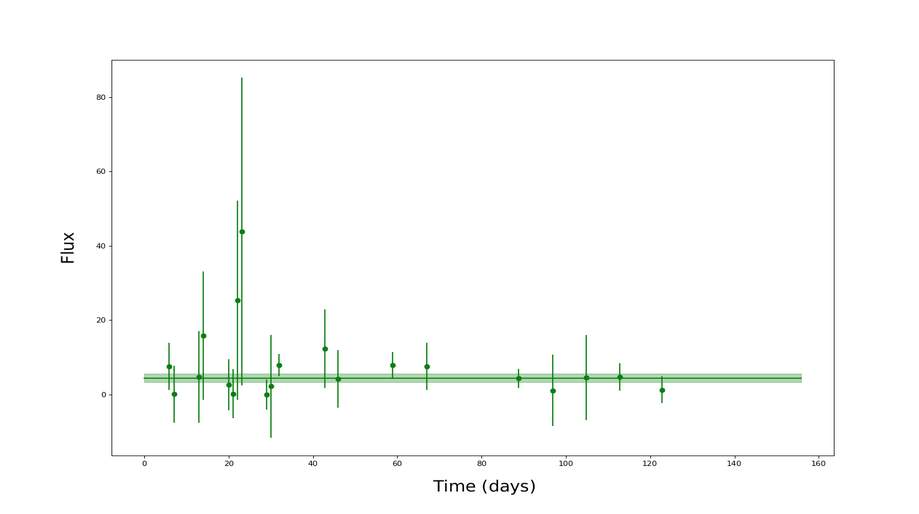
\includegraphics[width=15cm]{Ex_reta.png}
		\caption{Exemplo de interpolação não condizente com a realidade.}
		\label{fig:ExReto}
	\end{figure}
	
	\section{Delimitação}
	
	Todos os dados utilizados tanto neste trabalho quanto no artigo \cite{lochner}, foram extraídos da base de dados oferecida pelo desafio \citet{challenge}. A base de dados é de domínio público e pode ser obtida no repositório do desafio.
	
	Devido à granularidade dos dados brutos, foi necessário um pré-tratamento buscando apenas os dados que serão utilizados. Esse pré-tratamento foi aproveitado do pipeline do Instituto de Física da UFRJ, cujo processo visa ler os arquivos de texto transformando cada informação em uma chave de dicionário. 
	
	Ao fim dessa seleção de dados foram obtidos valores em forma de dicionários em Python para cada objeto astronômico. Esses dicionários serão os dados brutos dentro escopo deste trabalho.   
	
	\section{Objetivos}
	\label{sec:Obj}
	
	O objetivo do trabalho é otimizar determinados pontos do pipeline utilizado atualmente, após um estudo inicial ter sido feito para identificar pontos frágeis ou passíveis de melhoras.
	
	Esses pontos são apresentados e justificados a seguir, criando as três vertentes do projeto.
	
	\begin{itemize}
		\item Processo Gaussiano
		\item Aprendizagem Profunda
		\item Tratamento de Outliers		
	\end{itemize}
	
		\subsection{Processo Gaussiano \textit{Gaussian Process}}
		
		O Processo Gaussiano, é a primeira parte do tratamento após a transformação dos dados brutos em dicionários de Python. Está etapa será abordada no \autoref{chap:GP}.
		
		Cada objeto astronômico irá possuir uma quantidade de pontos que representam a intensidade do fluxo de luz captado em determinado dia, bem como a incerteza desse valor. Assim, busca-se uma interpolação para obter um gráfico que passe por determinados pontos. 
		
		O objetivo ao abordar esse ponto é consertar interpolações que não condizem com a interpretação física, como pode ser vista na figura \ref{fig:ExReto}.
		
		\subsection{Aprendizagem Profunda}		

		A Aprendizagem Profunda (\textit{Deep Learning} ou \textbf{DL}) vêm sendo um advento utilizado recentemente para aprimorar alguns algoritmos de Aprendizagem de Máquina (\textit{Machine Learning} ou \textbf{ML}). 
		
		A ideia de aplicar DL nesse problema veio a partir da análise do pipeline inicial. Tendo em vista que o mesmo possui diversas partes entre os dados brutos e algoritmo de Random Forest, busca-se aplicar DL esperando obter um pipeline mais simples, possuindo apenas uma etapa entre os dados brutos e o algoritmo de classificação.
		
		Em diversos outros casos na literatura, como identificação de sons ou imagens, houveram melhorias significativas ao reduzir o número de etapas envolvendo processamento de sinais (wavelets) ou redução de componentes (PCA) em troca do uso de DL. 
		
		A segunda motivação para a aplicação de DL veio do artigo da \citet{lochner}, onde ela menciona possíveis aplicações no escopo do problema.
		
		Assim, foi decidido aplicar algoritmos de DL após a primeira parte do tratamento de dados, visando manter uma simplicidade ao longo do pipeline, estabelecendo assim, apenas a etapa do GP entre os dados brutos e o algoritmo de classificação. O detalhamento desse procedimento encontra-se no \autoref{chap:DL}.

		\subsection{Tratamento de \textit{Outliers}}
		
		A última vertente para buscar melhorias no algoritmo é o tratamento de pontos cuja incerteza é muito alta ou cujos valores são fora do esperado, pontos com essas características são conhecidos na literatura como outliers.
		
		Analisando alguns dados brutos, e possível observar pontos cuja incerteza mostra-se mais de 100\% maior do que a própria curva (ponto mais a esquerda da figura \ref{fig:ExOutlierStd}) e também pontos que encontram-se completamente fora da curva interpolada \ref{fig:ExOutlier}.
		
		As etapas do tratamento encontram-se descritas no \autoref{chap:Out}.
		
		\newpage
		
		\begin{figure}[h!]
			\centering
			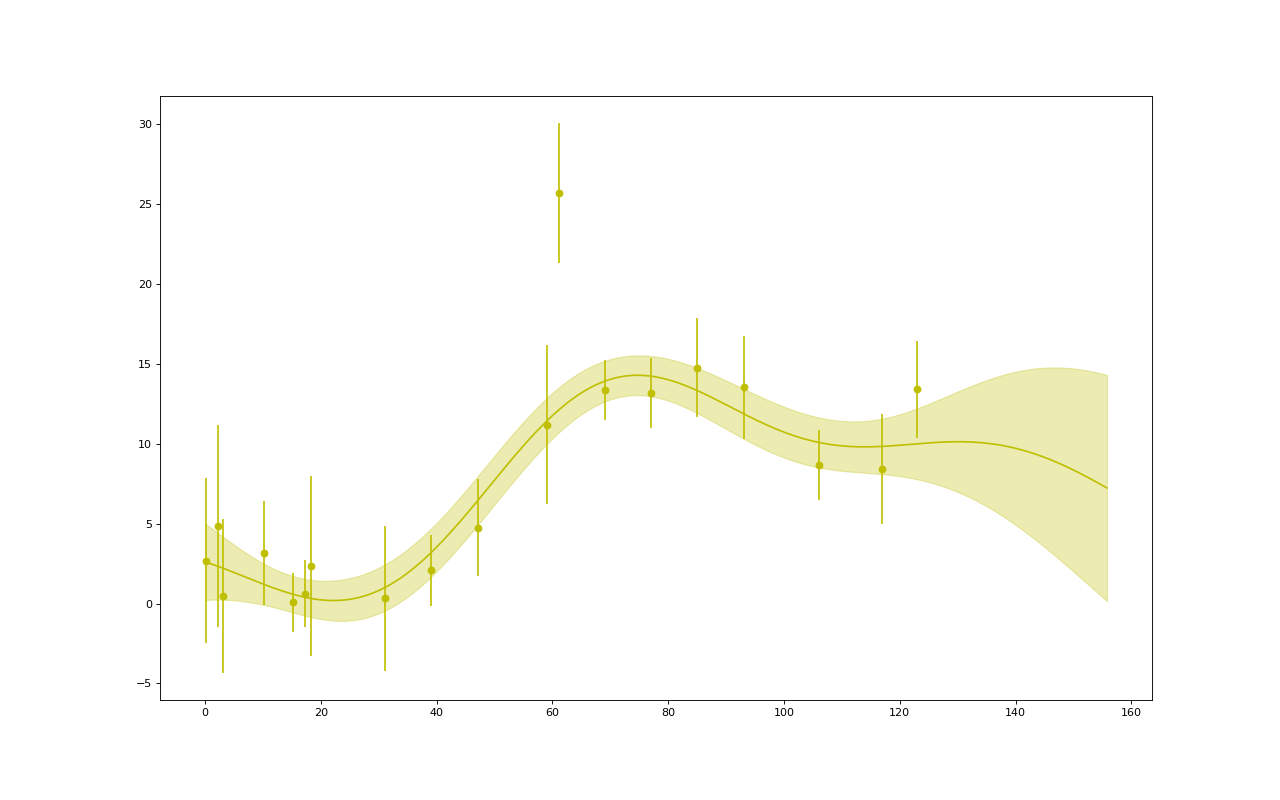
\includegraphics[width=15cm]{OutPoint.png}
			\caption[Exemplo de \textit{outlier}.]
			{{\small Exemplo de \textit{outlier}. Gráfico Fluxo $ \times $ Tempo (dias).}}
			\label{fig:ExOutlier}
		\end{figure}
	
		\begin{figure}[h!]
		\centering
		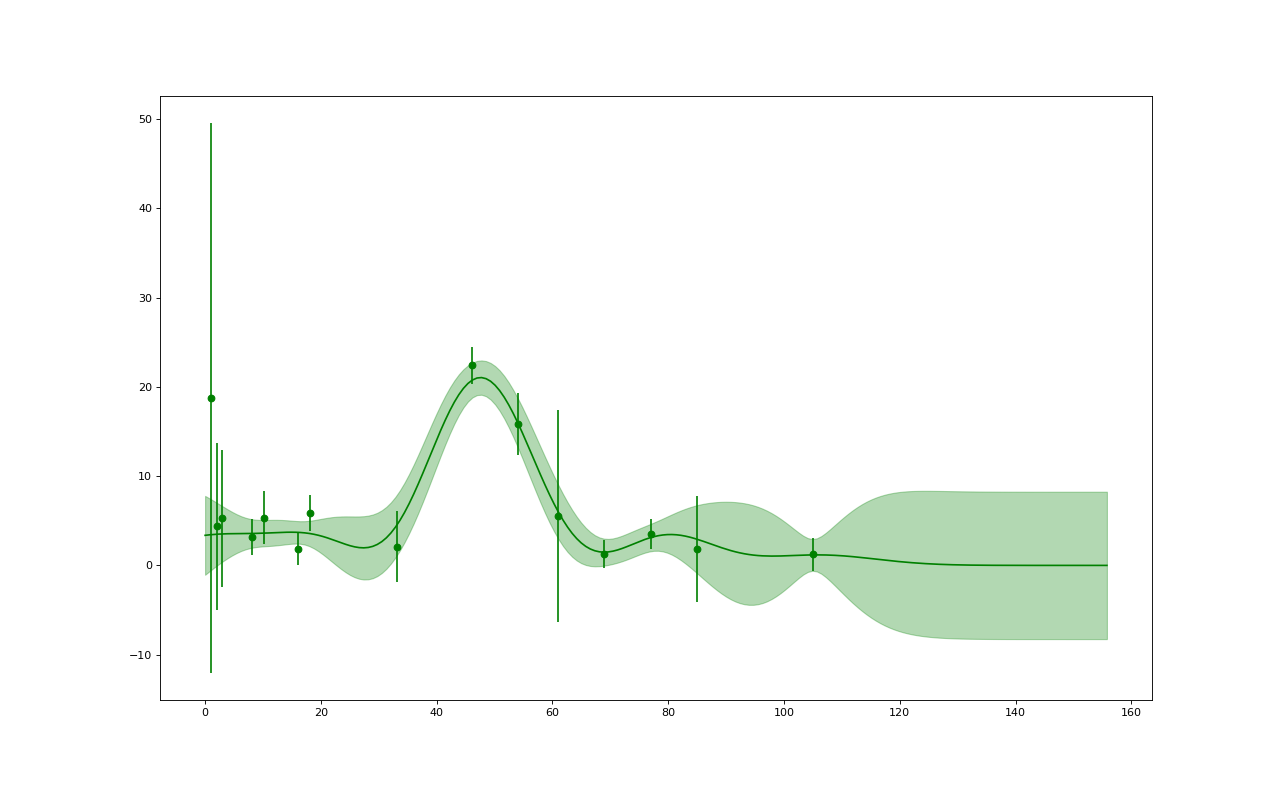
\includegraphics[width=15cm]{OutStd.png}
		\caption[Exemplo de ponto com incerteza 3 vezes maior que o pico da curva.]
		{{Exemplo de ponto com incerteza 3 vezes maior que o pico da curva. Gráfico Fluxo $ \times $ Tempo (dias).}}
		\label{fig:ExOutlierStd}
		\end{figure}
	

		
		\newpage

	\section{Metodologia}
	
	Devido ao código de pré-processamento do IF-UFRJ estar escrito em Python, todo o trabalho também foi escrito na mesma linguagem. Outro ponto para a sua escolha a facilidade que a mesma possui para realizar experimentos através da plataforma \textit{Jupyter}, além da grande quantidade de bibliotecas de ciência de dados e suporte para desenvolver algoritmos de ML. 
	
	As principais bibliotecas utilizadas no contexto de tratamento de dados foram \textit{Pandas} e \textit{Numpy}. Já para a aplicação dos métodos, as bibliotecas mais importantes foram \textit{scikit-learn}, \textit{Keras} e \textit{PyMC3}.
	
	A entrada dos modelos sempre serão os dicionários gerados a partir dos dados brutos após o pré-processamento do IF-UFRJ. Assim, pôde-se  filtrar com maior facilidade as propriedades desejadas para cada uma das três vertentes do trabalho. 

	Cada uma dessas vertentes possuiu um trabalho específico e isolado para poder melhor averiguar suas mudanças posteriormente. Em outras palavras, a cada mudança realizada houve a comparação direta com os resultados do pipeline original, de modo a poder avaliar especificamente a eficiência e melhora dessa mudança.
	
	Por se tratar de um algoritmo de classificação, a saída do modelo será booleana e classificará se um objeto astronômico é ou não do tipo IA. Entretanto, nos dados brutos, as classes são divididas em 8 tipos de objetos: \textit{IA, IB, IBC, IC, II, IIL, IIN} e \textit{IIP}.
	
	É importante ressaltar também que para validar os modelos do projeto foi usado o método \textit{K-fold}. Todavia, este trabalho se diferenciou da divisão clássica presente na literatura, normalmente uma divisão de 80\% dos dados para treinamento e 20\% para o teste dos modelos. Neste projeto foram utilizados apenas 1100 objetos para treino dentre 21316 objetos totais. A justificativa é a limitação física das amostras (espera se ter apenas 1100 objetos confirmados).
	
	Por fim, as mudanças foram verificadas através de \textbf{Matrizes de Confusão} (\textit{Confusion Matrices} ou \textbf{CM}) ou através de métodos de score da biblioteca \textit{scikit-learn}.
	
	Como última observação, a fim de estudos posteriores fora do escopo do projeto, foram feitas classificações envolvendo os 8 tipos de objetos, além de treinamentos adotando a proporção de 80\% para treino e 20\% para teste.
		
	\newpage
		
	\section{Descrição}
	No \autoref{chap:FundTeo}, serão explicados os principais conceitos teóricos utilizados na aplicação do \textbf{Processo Gaussiano} e no \textbf{Deep Learning}. Também serão levantados alguns conceitos não tão centrais do trabalho, mas de importância igualmente significativa.
	
	O \autoref{chap:ModeloAtual} será destinado para detalhar especificamente cada etapa do \textbf{pipeline atual}, assim como uma breve menção a maneira na qual os dados brutos são tratados.
	
	Os capítulos 4, 5 e 6 serão destinados à explicação dos \textbf{objetivos} citados na seção \ref{sec:Obj}, assim como os \textbf{resultados das mudanças} dos mesmos, buscando averiguar a eficiência de aplicação ou explicar possíveis erros.
	
	Por fim, no \autoref{chap:Concl} serão apresentadas as \textbf{conclusões finais do projeto e sugestões de trabalhos futuros}, junto às limitações e possíveis soluções encontradas.
	
	\newpage
	
  \chapter{Fundamentos Teóricos}
  \label{chap:FundTeo}
  
 	\section{Processo Gaussiano}
 	\label{sec:GP}
 	
 	O Processo Gaussiano é uma ferramenta importante para algoritmos de Machine Learning, pois permite fazer predições sobre os dados tendo como base um conhecimento a priori. A sua aplicação mais frequente é em interpolações de funções, como é o caso deste projeto. Há também possíveis aplicações do conceito em classificações e agrupamentos de grande quantidades de dados. O livro base utilizado para os estudos desse projeto foi \citet{GPBook} . 
 	
 	Sabendo que para uma quantidade determinada de pontos existe uma infinidade de funções que podem interpolar esses valores, o Processo Gaussiano realiza sua interpolação a partir dos conhecimentos a priori dos valores dessa função, assim como de um provável formato que ela pode assumir devido a relação entre seus pontos. Por fim, o GP não irá obter um valor específico para cada ponto da função interpolada, mas sim uma distribuição probabilística para cada ponto, onde cada um possuirá uma média (valor da interpolação) e um desvio padrão (incerteza).
 	
 	Neste projeto não são abordados maiores detalhes para o aprendizado do método, contudo, na bibliografia são encontradas tanto referências mais específicas e técnicas \cite{GPBook},   quanto mais práticas \cite{ridge}, \cite{GPDummies}, \cite{GPVisual}.
 	
 	Os dois aspectos fundamentais do Processo Gaussiano são os principais responsáveis por caracterizar as interpolações. Eles serão apresentados nas subseções a seguir.
 	
 	\newpage

	\subsection{\textit{Kernel} e Função de Covariância}
	
	O Processo Gaussiano interpola uma função discreta de $n$ pontos através dos $m$ pontos conhecidos, resultando em $n$ distribuições normais uma para cada ponto que irá constituir essa função discreta.
	
	Vale lembrar que uma função discreta cujos intervalos dos pontos do eixo das abscissas são significativamente pequenos, pode ser considerada contínua para efeitos práticos. 
	
	O diferencial do GP é considerar uma distribuição normal multivariável de dimensão $n+m$ durante a interpolação. Essa distribuição normal multivariável possuirá uma covariância $\Sigma$, responsável não por apenas descrever o \textbf{formato}, como também por determinar \textbf{características} da função a ser prevista.
	
	Para poder obter o $\Sigma$ desta normal multivariável é estabelecido o Kernel do GP. Ele é uma função de duas variáveis especial que respeita certas restrições matemáticas (Cap. 4 \citet{GPBook}). Essas varíaveis são os valores da abscissa de cada ponto da função a ser interpolada.
	
	Em outras palavras, o Kernel é uma função que irá relacionar dois pontos que deverão estar na curva interpolada, baseando se apenas na distância entre eles (para Kernels estacionários) ou nos seus valores absolutos (para Kernels não-estacionários). É essa relação que fornecerá características como periodicidade, picos e suavização da curva.
	
	É importante ressaltar que apenas os valores das abscissas serão utilizados para essa relação, enquanto os valores das ordenadas dos pontos conhecidos são utilizados para forçar que essa função passe por eles, através de \textbf{probabilidade condicionada} (\textit{\textbf{Posterior Distribution}} \cite{GPVisual}). Pode-se utilizar esse método de probabilidade condicionada devido à propriedade das distribuições gaussianas que afirma: distribuições condicionadas ou marginalizadas vindas de distribuições gaussianas também são gaussianas. 
	
	A figura \ref{fig:Kernel} ilustra uma maneira mais fácil de visualizar o que foi dito no parágrafo acima. Pode-se ver em \ref{fig:Kernel}(b) que os mesmos 10 pontos serão calculados já com a probabilidade condicionada para satisfazer os 2 pontos pré-estabelecidos.
	
	\begin{figure*}
		\centering
		\begin{subfigure}[h]{0.475\textwidth}
			\centering
			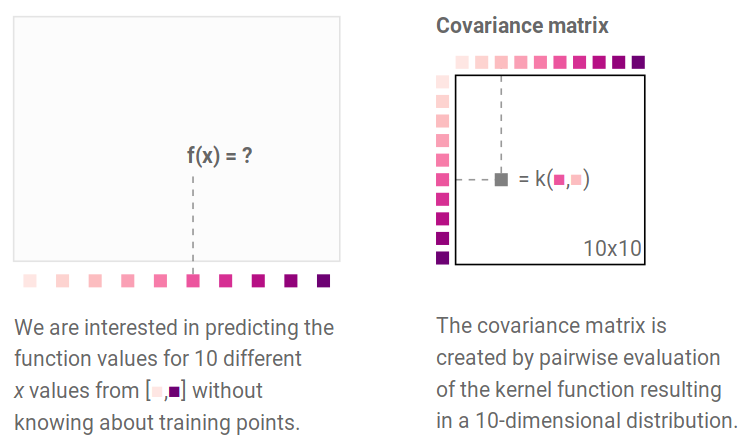
\includegraphics[width=1.1\textwidth]{Kernel1.png}
			\caption[]%
			{{\small Ilustração da matriz $\Sigma$ para 10 pontos.}}    
			\label{fig:Kernel1}
		\end{subfigure}
		\vskip\baselineskip
		\begin{subfigure}[h]{0.475\textwidth}   
			\centering 
			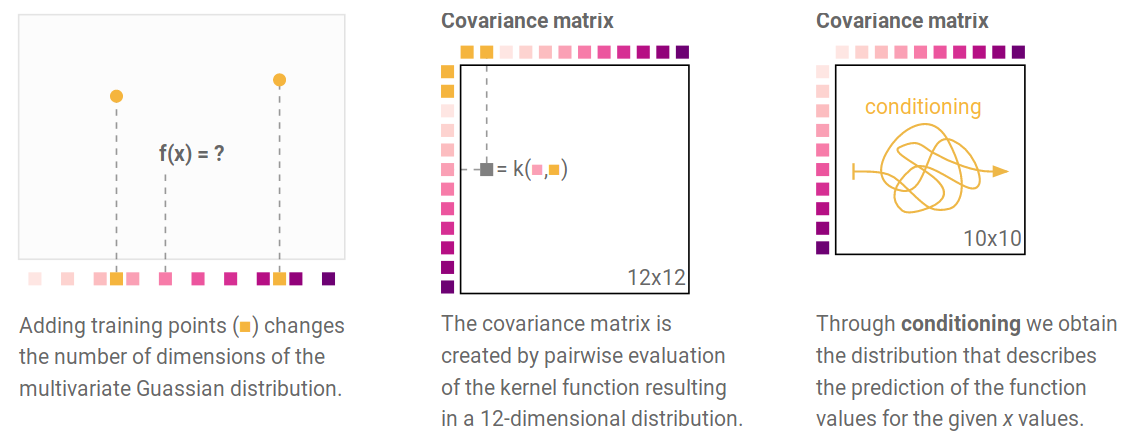
\includegraphics[width=1.1\textwidth]{Kernel2.png}
			\caption[]%
			{{\small Ilustração da matriz $\Sigma$ para 12 pontos. 2 deles são pontos dados.}}    
			\label{fig:Kernel2}
		\end{subfigure}
		\quad

		\caption[ Ilustração da matriz $\Sigma$ possuindo 10 e 12 pontos.]
		{\small Ilustração da matriz $\Sigma$ possuindo 10 e 12 pontos. \textit{Imagens retiradas de \citet{GPVisual}}} 
		\label{fig:Kernel}
	\end{figure*}
	
	\newpage
 	
 	\subsection{Função Média}
 	
 	A Função Média de um Processo Gaussiano é aquela responsável por oferecer a predição inicial do ponto a ser interpolado. É o valor que determinado ponto possuiria caso só existisse ele a ser definido.
 	
 	Contudo, só existe sentido em falar de função média caso seja associada à Função Covariância. Normalmente a Função Média é estabelecida como uma distribuição normal com média em 0 e desvio padrão 1. 
 	
 	É possível usar essa distribuição padrão como valor a priori pois, o valor final deste ponto será obtido após um número suficientemente grande de amostras para otimizar a distribuição. Elas são definidas através de amostragens usando \textbf{Cadeias de Markov Monte Carlo} \cite{MCMC}, se aproximando cada vez mais do valor ideal. No fim, o valor do ponto será a média dessa distribuição a posteriori. A figura \ref{fig:MCMC}(a) ilustra esse caso.
 	
 	Todavia, é imprescindível o uso correto da Função Média, pois caso ela tenha seu domínio delimitado, isso poderá impossibilitar que a função assuma alguns valores, como está ilustrado na \ref{fig:MCMC}(b).
 	
 	\begin{figure*}
 		\centering
 		\begin{subfigure}[h]{0.475\textwidth}
 			\centering
 			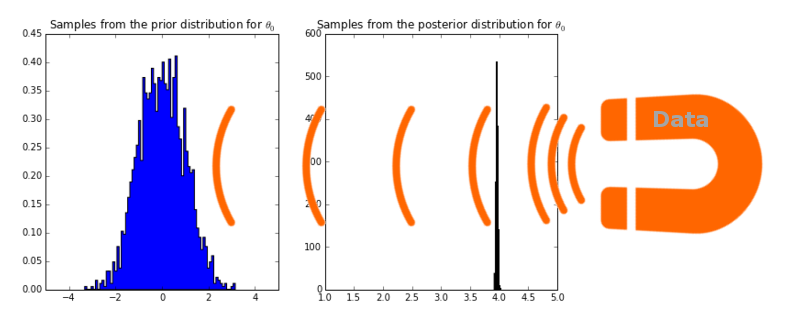
\includegraphics[width=1.1\textwidth]{mcmc1.png}
 			\caption[]%
 			{{\small Exemplo de priori gaussiana que ao longo das amostragens passa a assumir o valor real (no caso do exemplo é 4).}}    
 			\label{fig:MCMC1}
 		\end{subfigure}
 		\vskip\baselineskip
 		\begin{subfigure}[h]{0.475\textwidth}   
 			\centering 
 			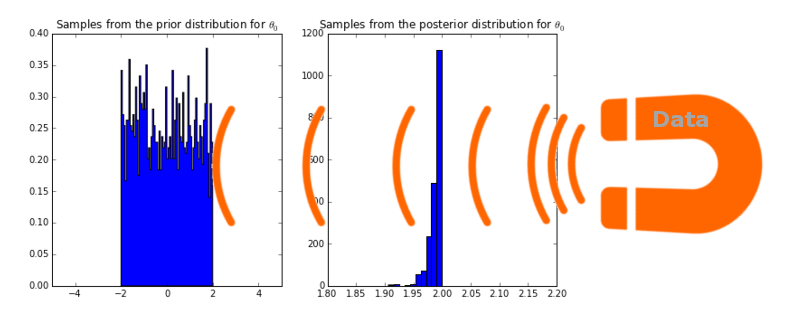
\includegraphics[width=1.1\textwidth]{mcmc2.png}
 			\caption[]%
 			{{\small Exemplo de priori delimitada que mesmo ao longo das amostragens nunca assumirá o valor real (no caso do exemplo é 4 e a delimitação é de -2 a 2).}}    
 			\label{fig:MCMC2}
 		\end{subfigure}
 		\quad
 		
 		\caption[ Ilustração do valor da função média.]
 		{\small Ilustração do valor da função média durante as amostragens via Cadeias de Markov Monte Carlo. \textit{Imagens retiradas da \citet{GPDummies}} } 
 		\label{fig:MCMC}
 	\end{figure*}
 	

 	
 	\section{Redes Neurais Convolucionais}
 	\label{sec:CNN}
 	
 	Redes Neurais Convolucionais (\textit{Convolutional Neural Network} \textbf{CNN}) são um tipo de rede neural em que \textit{Deep Learning} é aplicado, normalmente usado para análise de imagens. O principal objetivo dentro deste projeto é usar algoritmos de Machine Learning, logo, para evitar quaisquer confusões com as nomenclaturas, vale lembrar que DL se refere a uma técnica dentro da vasta área que é ML.\\
 	
 	Uma arquitetura básica de DL possui 3 partes \ref{fig:DLArch} :

 	
 	\begin{itemize}
 		\item \textit{Input Layer}: A primeira camada; aquela responsável por receber uma amostra do dado e repassar para as camadas internas

 		\item \textit{Hidden Layers}: O grupo de camadas internas; nela encontram-se os nós que recebem os dados da \textit{input layer} e conectam às camadas subsequentes através de funções de ativação não-lineares. 

 		\item \textit{Output Layer}: A última camada; responsável pela resposta final. Em uma rede de classificação ela possui valores de saída numéricos, referindo-se as classes. No caso deste projeto, são os números zero e um correspondendo as supernovas classificadas como \textit{IA} ou \textit{not IA}.

 	\end{itemize}
 
 	Cada camada é composta de diferentes tipos de \textbf{neurônios}. Eles são funções matemáticas com parâmetros específicos, os quais serão treinados a fim de classificar os dados.
 	
 	\begin{figure}[h!]
 		\centering
 		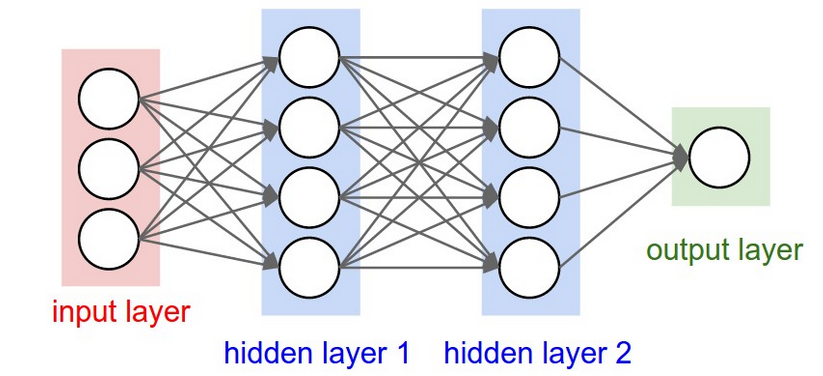
\includegraphics[width=12cm]{DLarch.png}
 		\caption[Arquitetura básica de \textit{Deep Learning}]
 		{{Arquitetura básica de \textit{Deep Learning}. (retirado de: \href{https://en.proft.me/2016/06/15/getting-started-deep-learning-r/}{link}.)}}
 		\label{fig:DLArch}
 	\end{figure}
 	
 	CNN é uma classe de redes neurais aplicada frequentemente na análise de imagens, neste projeto as imagens são arquivos \textit{png} criados através da interpolação gaussiana, que serão representados em formato de matrizes de valores, como pode ser visto na matriz azul da figura \ref{fig:convolution}. 
 	
 	Redes neurais convolucionais normalmente tratam-se de casos de redes totalmente conectadas, ou seja, cada neurônio em uma camada é conectado em todos os neurônios a camada seguinte. Essa alta conectividade faz com que o algoritmo demande o mínimo de pré-processamento possível quando comparada a outros métodos de classificação de imagens, pois caso sejam dadas amostras o suficiente, a rede ''aprende'' os filtros que em um algoritmo tradicional precisariam ser implementados manualmente \cite{wikiCNN}. Nas CNN também são usados \textit{multilayers perceptrons} \cite{wikiperceptron}, a função de cada neurônio pode ser entendida como a ilustração da matriz verde na figura \ref{fig:convolution} e cada parâmetro sendo o número que multiplica o valor da matriz azul.

		\newpage

 	\begin{figure}[h!]
		\centering
		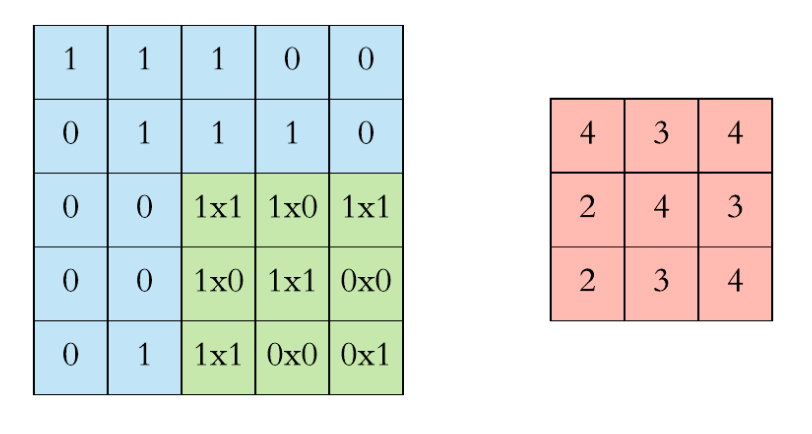
\includegraphics[width=12cm]{convolution.png}
		\caption[Operação de Convolução.]
		{{A matriz azul representa as variáveis de entrada; a vermelha os resultados da operação de convolução; e a verde possui os parâmetros para multiplicar valores da matriz azul ''deslizando'' através deles. (retirado de: \href{https://towardsdatascience.com/applied-deep-learning-part-4-convolutional-neural-networks-584bc134c1e2}{link}.)}}
		\label{fig:convolution}
	\end{figure}
 	
	CNNs podem possuir camadas de conjugação \textit{pooling}, responsáveis por particionar retângulos da imagem de entrada em um conjunto menor de pixels para cada sub região. Dentre diversas funções \textit{pooling} não-lineares, a mais usada é a de \textit{max pooling} \ref{fig:maxpooling}. 
 	
 	\begin{figure}[h!]
 		\centering
 		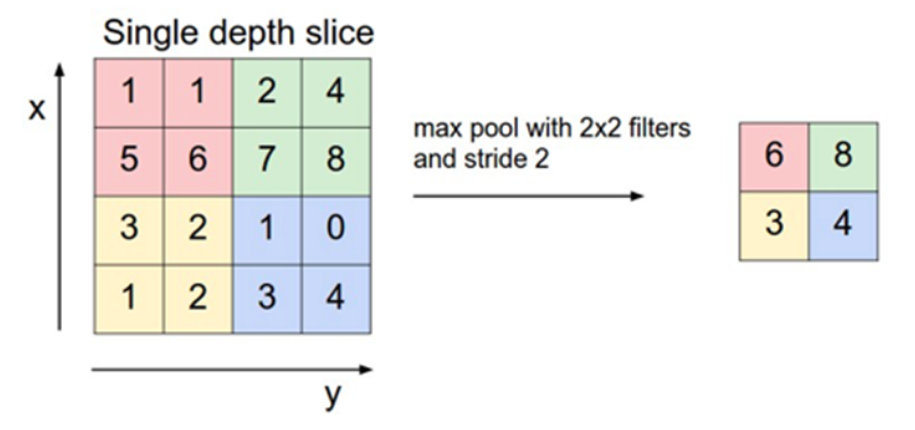
\includegraphics[width=12cm]{maxpooling.png}
 		\caption[\textit{Max Pooling.}]
 		{{Exemplo do \textit{Max pooling}, o maior valor dentro de um ''retângulo'' é selecionado e propagado para outra camada, esta possuindo sua dimensão reduzida (retirado de: \href{http://cs231n.github.io/convolutional-networks/\#pool}{link}.)}}
 		\label{fig:maxpooling}
 	\end{figure}

 	Dentro das camadas internas é impossível de afirmar precisamente qual o ''sentido físico'' de cada uma. Algumas podem possuir apenas significado matemático enquanto outras podem ser responsáveis por identificar pontas, olhos, pés, curvas, etc. 
 	
 	\newpage

 	É importante mencionar que existe um pequeno fator de aleatoriedade dentro dos processos de treinamento envolvendo a otimização dos parâmetros internos de cada neurônio. Para estabelecer uma comparação livre de possíveis erros causados pela aleatoriedade, foram usadas \textit{random seeds}, funções do Python responsáveis por conservar a pseudoaleatoriedade \cite{pseudoaleatoriedade}. 

 	\section{Demais Conceitos}
 	\label{sec:OtherConcepts}
 	
 	Aqui estão apresentados alguns conceitos menos usados ao longo do pipeline.
 		
 		\subsection{Análise de Componentes Principais}
 		
 		A Análise de Componentes Principais (Cap. 12 \citet{ML}) ou \textit{Principal Component Analysis} (\textbf{PCA}) utiliza conceitos de ortogonalizações de vetores para poder reduzir dimensões.
 		
 		Em ML essa redução de dimensões é aplicada às features de um dataframe onde as amostras possuem um grande número de características e deseja reduzi-las, com a finalidade de que o modelo de aprendizagem de máquina seja menos custoso e igualmente eficaz.
 		
 		Através de técnicas vindas da álgebra linear, o método ''cria'' novas dimensões virtuais compostas por combinações lineares das já existentes, de maneira que estas novas dimensões poderão melhor distinguir a quantidade de dados existentes no dataframe. 
 		
 		Por fim pode-se também interpretar PCA através de uma perspectiva de filtros, onde se decompõe determinado sinal e selecionando determinadas frequências conserva-se a potência dele. Por essa perspectiva, as frequências são as features e a potência é a capacidade que as novas features têm de representar o dataframe.
 		
 		\subsection{Transformadas de \textit{Wavelet}}
 		
 		Transformadas de \textit{Wavelet} \cite{Afonso} ou onduletas são funções capazes de descrever ou representar outras funções em diferentes escalas de frequência e de tempo.
 		
 		São normalmente usadas no domínio de processamento de sinais, sendo úteis para eliminar ruídos e comprimir dados, por exemplo.
 		
 		Neste projeto as Transformadas de \textit{Wavelet} servem para processar os gráficos interpolados do GP. Resultando assim em valores que podem ter possíveis erros de interpolação eliminados. 
 		
  		\subsection{Validação cruzada \textit{K-Fold}}
  		
  		Validação cruzada é uma família de métodos estatísticos usada para estimar como um modelo pode ser generalizado independente do conjunto de treino e teste. Em suma, é comumente utilizada para analisar se um modelo é robusto o suficiente, assim como para analisar a quantidade de falsos positivos e falsos negativos. Validação Cruzada \textit{K-Fold} é um desses métodos.
  		
  		Seu procedimento consiste em dividir os dados em $K$ partes, \textbf{normalmente} $K-1$ são utilizados para treinar o modelo, enquanto $1$ é usado para teste. Todavia, neste projeto devido as limitações físicas, apenas uma parte será usada para o treino enquanto as demais dezoito serão utilizadas para testar e validar o método.
  		
  		Junto a validação cruzada existem 2 conceitos que serão usados para avaliar os resultados deste projeto
  		
  		\begin{itemize}
  			\item Curva ROC e AUC (Cap. 5.7 \citet{ML})
  			\item \textit{Mean Average Precision} (Cap. 9.7.4 \citet{ML})
  		\end{itemize}
  	
  		 
  		
	\newpage
  \chapter{Modelo Atual}
  \label{chap:ModeloAtual}  		
  
  Neste capítulo serão detalhados o modelo atualmente utilizado para estudos cosmológicos do IF-UFRJ.


	\section{Pré-processamento dos Dados Brutos}
	
	Os dados brutos chegam da seguinte forma para o pré-processamento \ref{fig:RawData}.
	
	
	\begin{figure}[ht]
		\centering
		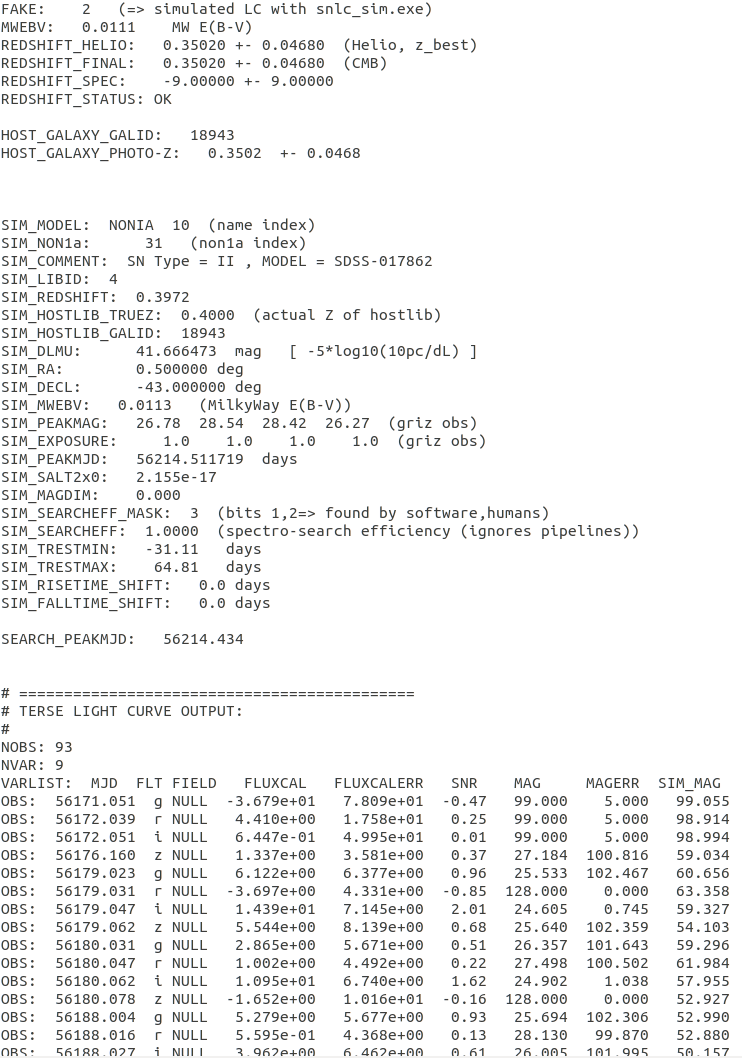
\includegraphics[width=9cm]{raw_dat.png}
		\caption{Arquivo \textit{.txt} a ser lido pelos arquivos de pré-processamento.}
		\label{fig:RawData}
	\end{figure}
	
	A partir  dos arquivos de pré-tratamento serão obtidas todas essas informações em forma de dicionário, entretanto, apenas as seguintes serão utilizadas durante o projeto.
	
	\begin{itemize}
		\item \textbf{SN TYPE} : Informa o tipo de supernova
		\item  \textbf{TERSE LIGHT CURVE OUTPUT} : Informa os pontos observados. Será o data frame. 
		\begin{itemize}
			\item \textbf{MJD} : O momento em que a observação foi obtida. A medida está descrita em dias do calendário Juliano.
			\item \textbf{FLT} : O filtro no qual a observação foi obtida, tendo em vista que os objetos são observados em 4 espectros de luz. 
			\item  \textbf{FLUXCAL} : O valor do fluxo de luz obtido naquela observação.
			\item  \textbf{FLUXCALERR} : O valor do erro do fluxo de luz.
		\end{itemize}
	\end{itemize}

	Em relação ao \textbf{MJD} vale explicar que é um método usado na astronomia para contar os dias sequencialmente começando em uma data arbitrária no passado. Neste projeto essas datas serão normalizadas, tendo como 0 o menor valor do MJD para que o eixo das abscissas tenha sempre início em 0.

	Em relação ao \textbf{FLT}, cada objeto astronômico é visto através de 4 filtros de luz diferentes, obtendo assim 4 curvas de luz para cada um deles. Na perspectiva de aprendizagem de máquina cada objeto possuirá 4 data frames, um para cada filtro, e posteriormente essas propriedades serão convertidas em features de cada objeto.
	
	A figura \ref{fig:ExFiltro} ilustra as 4 curvas de luz para o mesmo objeto.
	
	\begin{figure*}
		\centering
		\begin{subfigure}[b]{0.475\textwidth}
			\centering
			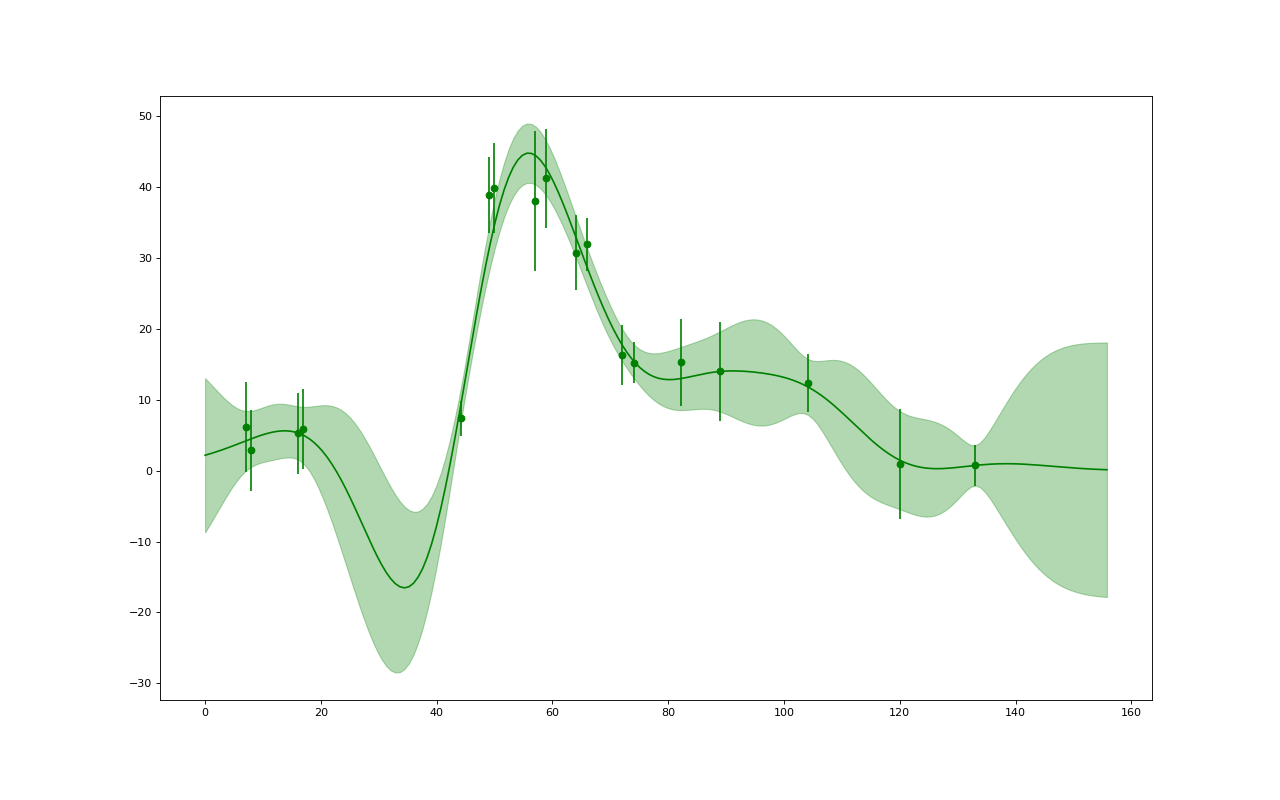
\includegraphics[width=\textwidth]{SN000017_II_desg.png}
			\caption[]%
			{{\small Filtro \textit{desg}}}    
			\label{fig:mean and std of net14}
		\end{subfigure}
		\hfill
		\begin{subfigure}[b]{0.475\textwidth}  
			\centering 
			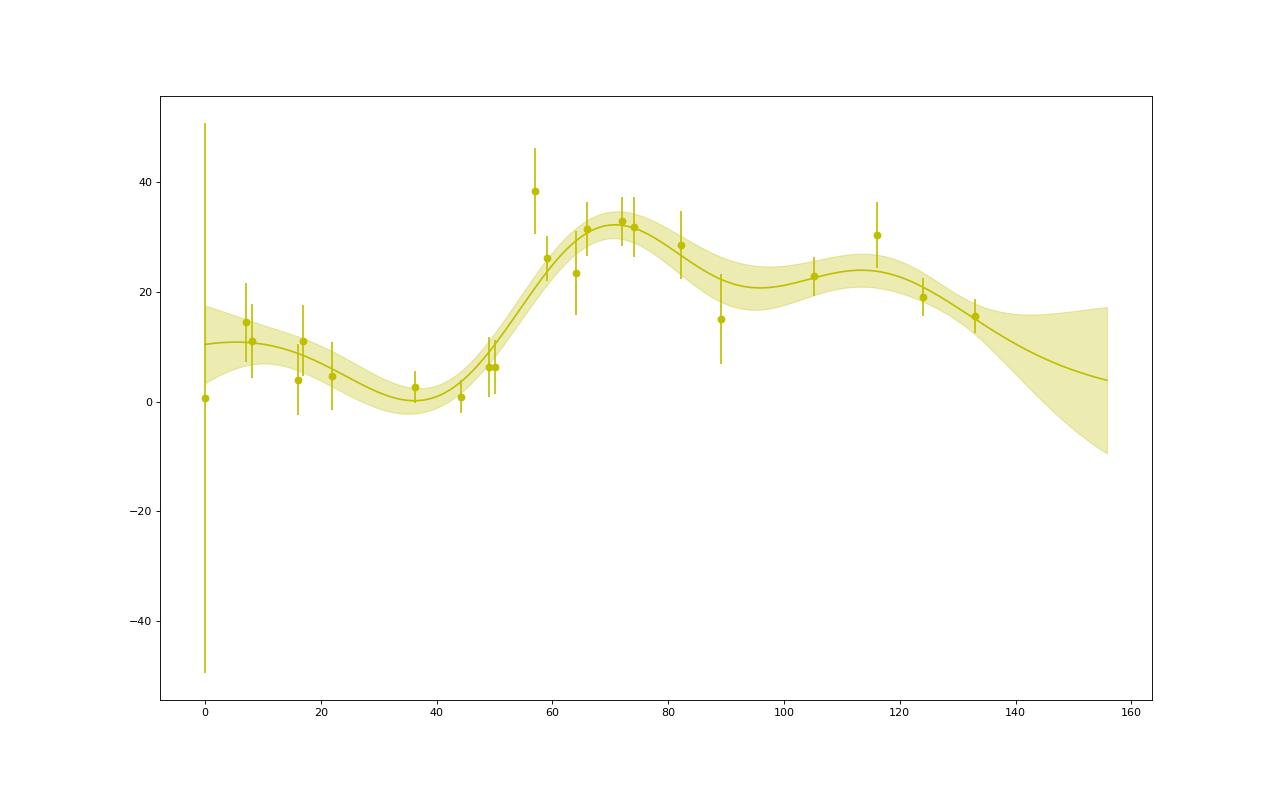
\includegraphics[width=\textwidth]{SN000017_II_desi.png}
			\caption[]%
			{{\small Filtro \textit{desi}}}    
			\label{fig:mean and std of net24}
		\end{subfigure}
		\vskip\baselineskip
		\begin{subfigure}[b]{0.475\textwidth}   
			\centering 
			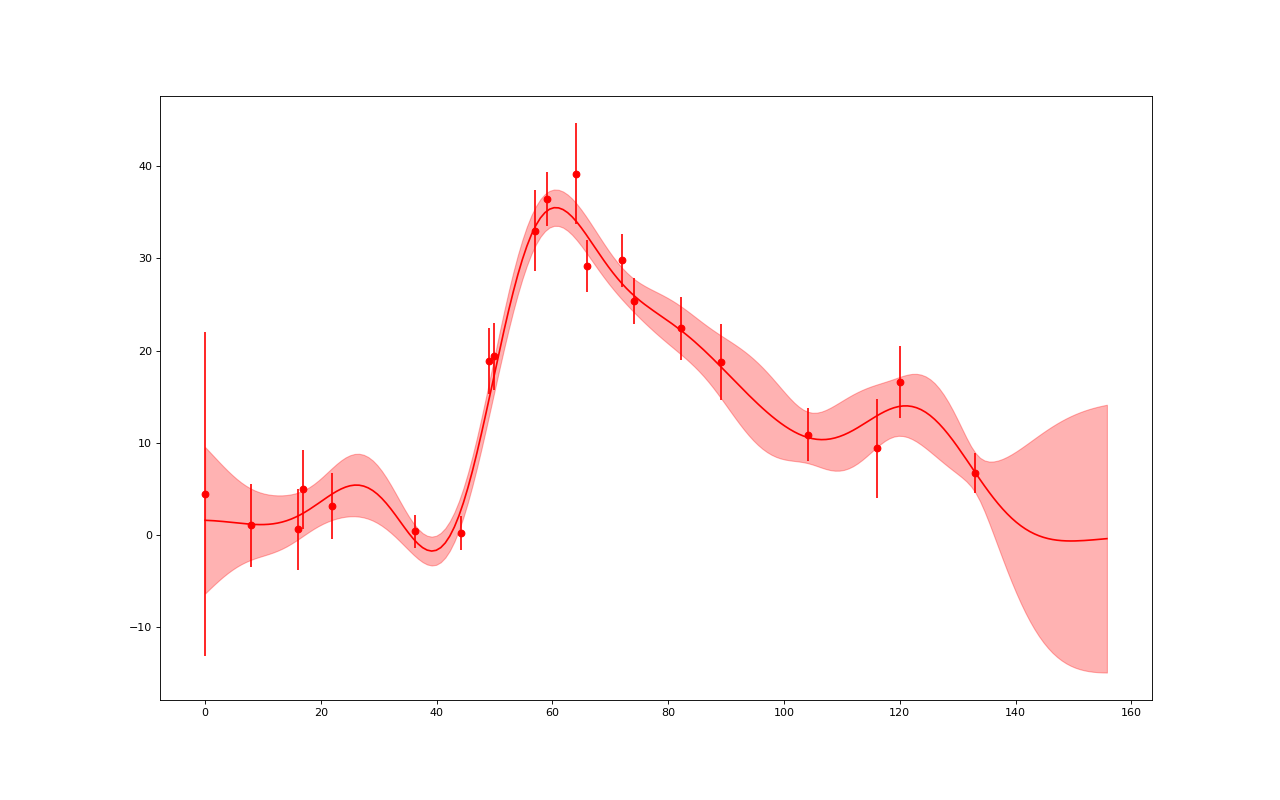
\includegraphics[width=\textwidth]{SN000017_II_desr.png}
			\caption[]%
			{{\small Filtro \textit{desr}}}    
			\label{fig:mean and std of net34}
		\end{subfigure}
		\quad
		\begin{subfigure}[b]{0.475\textwidth}   
			\centering 
			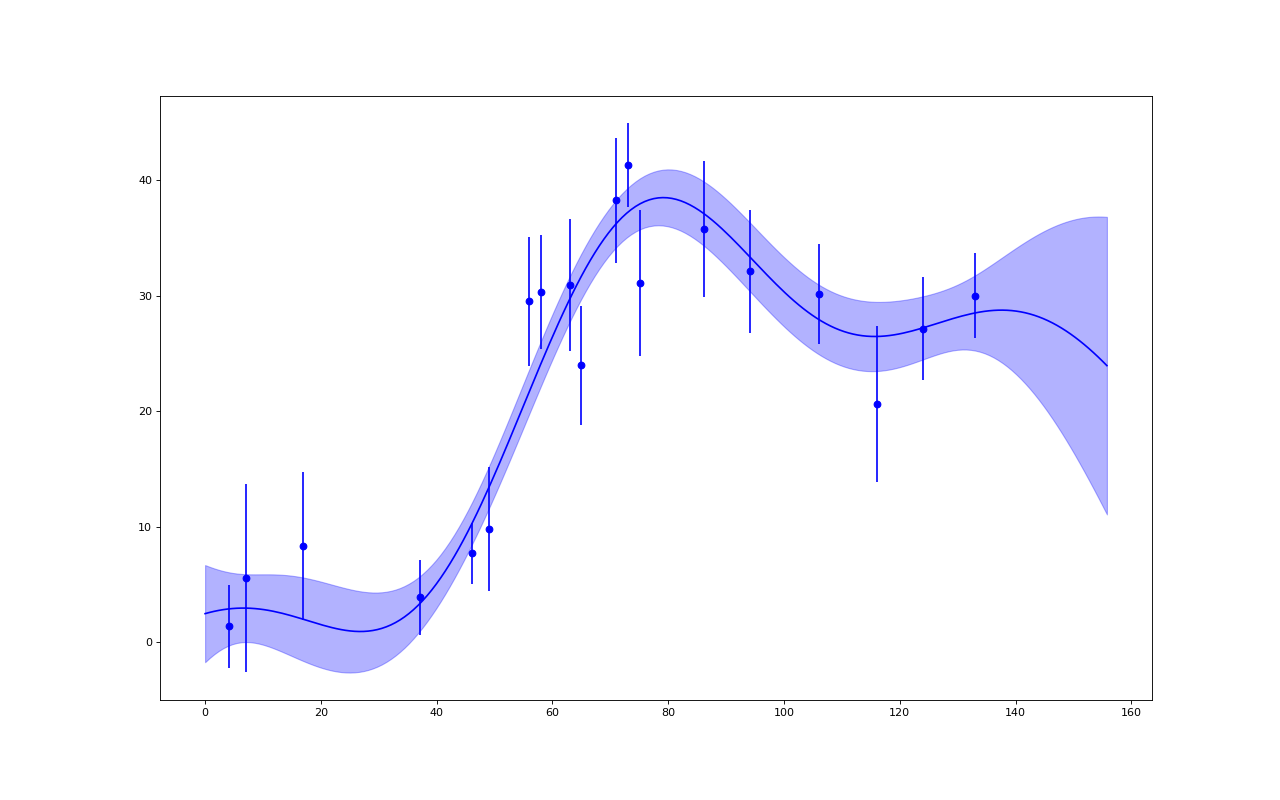
\includegraphics[width=\textwidth]{SN000017_II_desz.png}
			\caption[]%
			{{\small Filtro \textit{desz}}}    
			\label{fig:mean and std of net44}
		\end{subfigure}
		\caption[ Exemplo de 4 curvas de luz de um mesmo objeto.]
		{\small Exemplo de 4 curvas de luz de um mesmo objeto, uma para cada filtro. Gráfico Fluxo $ \times $ Tempo (dias).} 
		\label{fig:ExFiltro}
	\end{figure*}
	
	\section{\textit{Pipeline} Atual}
	
	Dispondo dos dados obtidos pelo pré-processamento explicado na seção anterior, inicialmente o pipeline irá separar os dados do \textit{Terse Light Curve Output} pelos filtros e irá criar 4 \textit{numpy arrays} possuindo $n \times 3$ dimensões cada (\textbf{MJD}, \textbf{FLUXCAL} e \textbf{FLUXCALERR}), sendo n o número de amostras.
	
	Em seguida, esses 4 \textit{numpy arrays} serão a entrada do Processo Gaussiano, cuja função é interpolar uma curva que passe pelos pontos de cada filtro \ref{fig:ExFiltro}.
	
	\newpage
	
	A saída do Processo Gaussiano será o gráfico interpolado em forma de \textit{numpy array} $100 \times 3$, contendo 100 pontos de abscissa, 100 pontos de ordenada e 100 pontos do erro da ordenada. 
	
	Essa saída será a entrada do processo de \textit{wavelets}, que irá retornar 400 valores para cada entrada. 
	
	No total esse procedimento se repetirá quatro vezes para cada objeto, uma para cada filtro. Assim, como saída do processo de \textit{wavelets} serão 1600 coeficientes para cada objeto astronômico.
	
	Em seguida é realizada uma redução de variáveis através da \textbf{análise de componentes principais} resultando em cada objeto com 20 features.
	
	Após essa etapa, o dataframe estará composto por 21316 amostras com 20 features cada.
	
	Em paralelo, usa-se o \textbf{SN TYPE} do dicionário para armazenar os tipos (labels) de cada objeto astronômico em forma de lista.
	
	Finalmente serão estabelecidos os parâmetros que caracterizam o modelo de classificação baseado em \textit{Random Forest}. Neste ponto é usado o módulo \textit{sklearn.pipeline} da biblioteca \textit{scikit-learn}.
	
	Tendo em mãos o dataframe, a lista com as classificações de cada objeto (os labels) e o modelo de classificação, é feita a divisão através do método \textit{k-fold} de validação cruzada, dividindo os objetos em 19 partições e usando 1 delas para treino e as demais para teste.
	
	Por fim cada modelo dos 19 \textit{folds} existentes é avaliado através de 2 maneiras de obtenção de score, o \textbf{método AUC} e o \textbf{método de precisão média} \ref{sec:OtherConcepts}. As matrizes de confusão de cada um dos 19 modelos também podem ser analisadas para ilustrar seus acertos, falsos positivos e falsos negativos \ref{fig:CMEx}. 

	\begin{figure*}[h]
	\centering
	\begin{subfigure}[b]{0.475\textwidth}
		\centering
		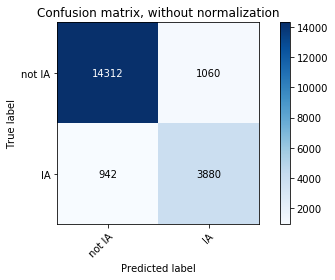
\includegraphics[width=\textwidth]{cm_ex.png}
		\caption[]%
		{{\small Exemplo de Matriz de Confusão, valores absolutos.}}    
		\label{fig:CMExValor}
	\end{subfigure}
	\hfill
	\begin{subfigure}[b]{0.475\textwidth}  
		\centering 
		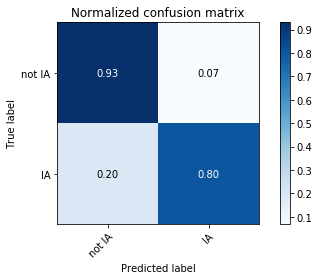
\includegraphics[width=\textwidth]{cm_exp.png}
		\caption[]%
		{{\small Matriz de Confusão, valores normalizados.}}    
		\label{fig:CMExPorcentavem}
	\end{subfigure}
	\caption[ Matrizes de Confusão de um modelo final do \textit{pipeline} original. ]
	{\small Matrizes de Confusão do modelo final do pipeline original.} 
	\label{fig:CMEx}
	\end{figure*}
	
	\newpage
  \chapter{Tratamento de Outliers}
  \label{chap:Out}
  
  	A primeira forma de buscar melhorias neste projeto foi o tratamento de Outliers. Todos os tipos de dados brutos estão sujeitos a amostras com valores absurdos ou incertezas irreais, sejam elas causadas por erros de medição ou quaisquer outros fatores \cite{Erros}.
  
 	\section{Estratégias Utilizadas}  	
 	
 	O primeiro tratamento realizado foi a retirada de pontos negativos. Visto que os valores a serem interpolados são fluxos de luz em função do tempo, não há sentido físico em haver pontos negativos.
 	
 	A segunda estratégia foi analisar a incerteza das amostras de cada ponto referente aos 4 filtros dos objetos astronômicos. Em seguida, foi calculada a \textbf{média} e o \textbf{desvio padrão} desses conjuntos de incertezas e por fim, houve a exclusão daqueles pontos cujo erro era superior à média mais um desvio padrão da distribuição de incertezas.
 	
 	Outra tentativa foi a aplicação de limiares baseados nos valores das incertezas de cada ponto em relação ao pico da curva. Caso o valor da incerteza fosse maior que o pico da curva multiplicado por um limiar (valor entre 0 e 1), este ponto seria excluído.
 	
 	O código referente a implementação deste tratamento de outlier, assim como todo o código do projeto, encontra-se disponível no \textit{GitHub} \ref{chap:Apendice}.
 	
 		\newpage
 		
 	\section{Resultados e comparações}
 	
 	Serão apresentados 3 tipos diferentes de scores para cada um dos 19 modelos gerados pela validação cruzada K-Fold: curva AUC (\textbf{AUC}), \textit{Average Precision} (\textbf{AP}) e o padrão da biblioteca \textit{scikit}; tendo sido aplicadas as seguintes estratégias:
 	
 	\begin{itemize}
		\item Retirada de valores negativos e daqueles com incerteza maior que a média mais desvio padrão. Representada na tabela \ref{tab:outlier} como \textbf{StdDev}.
		\item Retirada de valores negativos e daqueles com incerteza maior do que 70\% do valor do pico. Representada na tabela \ref{tab:outlier} como \textbf{Threshold}.
 	\end{itemize}


 	\begin{table}[h!]
 		
 		\begin{center}	
 			\small\addtolength{\tabcolsep}{-5pt}
 			\begin{tabular}{|l|c|c|c|c|c|c|c|c|c|} % <-- Alignments: 1st column left, 2nd middle and 3rd right, with vertical lines in between
 	\hline
Fold & \textbf{AUC} & \textbf{\makecell{AUC \\ StdDev}} & \textbf{\makecell{AUC \\ Threshold}} & \textbf{AP} & \textbf{\makecell{AP \\ StdDev}} & \textbf{\makecell{AP \\ Threshold}}& \textbf{Padrão} & \textbf{\makecell{Padrão \\StdDev}} & \textbf{\makecell{Padrão \\ Threshold}}\\

\hline
\small{Fold 1 }&   95,93\% &95,18\%& 95,99\%& 86,34\% & 83,86\% & 86,41\% & 90,33\%& 89,65\%& 90,35\%\\
\small{Fold 2 }&   95,76\% &94,88\%& 95,75\%& 84,51\% & 81,72\% & 84,36\% & 90,11\%& 89,00\%& 90,09\%\\
\small{Fold 3 }&   96,02\% &94,89\%& 96,01\%& 87,25\% & 82,93\% & 87,27\% & 90,70\%& 89,14\%& 90,51\%\\
\small{Fold 4 }&   95,65\% &94,77\%& 95,71\%& 84,73\% & 81,99\% & 84,96\% & 89,68\%& 88,47\%& 89,46\%\\
\small{Fold 5 }&   95,72\% &95,01\%& 95,86\%& 85,34\% & 83,42\% & 86,34\% & 90,19\%& 89,51\%& 90,11\%\\
\small{Fold 6 }&   95,79\% &94,81\%& 95,68\%& 84,27\% & 82,30\% & 84,04\% & 90,42\%& 88,97\%& 90,26\%\\
\small{Fold 7 }&   95,56\% &94,82\%& 95,93\%& 85,20\% & 83,75\% & 86,36\% & 89,73\%& 88,96\%& 90,36\%\\
\small{Fold 8 }&   95,82\% &95,19\%& 95,90\%& 85,49\% & 84,12\% & 86,10\% & 90,00\%& 89,41\%& 90,25\%\\
\small{Fold 9 }&   95,74\% &95,24\%& 95,93\%& 85,71\% & 83,66\% & 86,87\% & 90,27\%& 89,45\%& 90,40\%\\
\small{Fold 10} &  95,91\% &94,96\%& 95,94\%& 87,38\% & 85,24\% & 87,52\% & 90,65\%& 89,76\%& 90,69\%\\
\small{Fold 11} &  95,89\% &95,42\%& 95,95\%& 85,90\% & 84,63\% & 86,77\% & 90,19\%& 89,61\%& 90,33\%\\
\small{Fold 12} &  95,72\% &94,81\%& 95,93\%& 85,02\% & 81,56\% & 86,06\% & 90,19\%& 89,06\%& 90,46\%\\
\small{Fold 13} &  95,69\% &95,29\%& 95,85\%& 85,19\% & 83,69\% & 85,86\% & 89,82\%& 89,55\%& 89,99\%\\
\small{Fold 14} &  95,48\% &94,81\%& 95,51\%& 84,65\% & 82,17\% & 85,06\% & 89,83\%& 88,84\%& 89,94\%\\
\small{Fold 15} &  95,65\% &95,29\%& 95,66\%& 84,84\% & 84,56\% & 85,68\% & 89,91\%& 90,18\%& 90,26\%\\
\small{Fold 16} &  95,83\% &95,55\%& 95,95\%& 86,48\% & 85,30\% & 86,56\% & 90,12\%& 89,79\%& 90,00\%\\
\small{Fold 17} &  96,01\% &95,41\%& 95,97\%& 86,19\% & 84,58\% & 85,95\% & 90,28\%& 89,66\%& 90,19\%\\
\small{Fold 18} &  95,96\% &95,47\%& 95,86\%& 85,84\% & 83,88\% & 85,55\% & 90,63\%& 90,02\%& 90,60\%\\
\small{Fold 19} &  95,35\% &95,37\%& 95,47\%& 84,34\% & 84,16\% & 84,47\% & 89,87\%& 89,61\%& 89,70\%\\
\hline
\hline
\textbf{Média} &  \textbf{95,76\%} & \textbf{95,11\%} & \textbf{95,83\%} & \textbf{85,51\%} & \textbf{83,55\%} & \textbf{85,90\%} & \textbf{90,15\%} & \textbf{89,40\%} & \textbf{90,21\%} \\
\hline
 			\end{tabular}
 		\end{center}
 	\caption{Resultados do tratamento de \textit{outliers}.}
 	\label{tab:outlier}
 	\end{table}
	
	\normalsize
	
 	A conclusão final para o tratamento de outliers é que o mesmo não influencia significativamente no aumento dos scores, a possível explicação para isto encontra-se na robustez que as transformadas de wavelets oferecem ao método.
 	
	\newpage 		
  \chapter{Rede Neural Convolucional}
  \label{chap:DL}
 	
 	 \section{Geração de Imagens e Parâmetros}  
 	 
 	 A primeira etapa desta abordagem consiste em gerar gráficos a partir da interpolação gaussiana. Para poder comparar o resultado deste método com o do pipeline inicial, a interpolação realizada para gerar os gráficos fornecidos ao modelo de Deep Learning foi a mesma interpolação usada no pipeline original.
 	 
 	 Estes gráficos serão imagens em escalas de cinza na extensão \textit{png}, cujas dimensões são: $64 \times 40$ pixels. Ao gerar essas imagens eram criadas margens com 5 pixels na dimensão $y$ e 9 pixels na dimensão $x$. No fim, elas foram eliminadas resultando em um formato de dimensão $46 \times 30$.
 	 
 	 Esses tamanhos foram escolhidos baseando-se em exemplos clássicos e bem conhecidos da literatura que possuem dimensões com valores bem próximos, como o \href{	https://towardsdatascience.com/image-classification-in-10-minutes-with-mnist-dataset-54c35b77a38d
 	 }{MNIST} e \href{https://github.com/zalandoresearch/fashion-mnist}{Fashion MNIST}.

 	\section{Pipeline} 	
 	
 	Após a transformação dos arquivos de imagem para matrizes de \textit{numpy array}, foi construída uma estrutura de dados para cada objeto como um compilado de suas 4 figuras. Obtendo o formato final de \textbf{(21316, 4, 30, 46)}, onde:
 	\begin{itemize}
 		\item Número de objetos: 21316
		\item Número de imagens ou matrizes (referente a cada filtro): 4
		\item Número de pixels por coluna (ou número de linhas): 30
		\item Número de pixels por linha (ou número de colunas): 46   
		
 	\end{itemize}
 
 	Dentre diversos possíveis tipos de camadas internas de Deep Learning, foram escolhidas camadas do tipo \textbf{Convolucionais 2D} e \textbf{\textit{Max Pooling} 2D} (seção \ref{sec:CNN}).
 	
 	A arquitetura escolhida também foi baseada em exemplos clássicos de problemas de identificação de imagens, em especial o \href{https://github.com/zalandoresearch/fashion-mnist}{Fashion MNIST}.
 	
 	Tendo como base esses exemplos, algumas camadas foram adicionadas e modificadas de forma a buscar empiricamente obter um melhor resultado. A arquitetura final encontra-se na figura \ref{fig:DLArchUsed}. 
 	
 	\begin{figure}[ht]
 		\centering
 		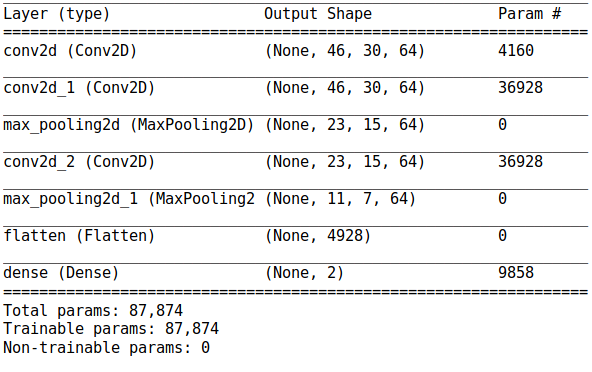
\includegraphics[width=11cm]{DL_architecture.png}
 		\caption{Arquitetura do modelo de Deep Learning utilizado.}
 		\label{fig:DLArchUsed}
 	\end{figure}
 
 	O último valor do \textit{Shape} de cada camada é a quantidade de neurônios que ela possui, enquanto os demais valores são o número de linhas e colunas da imagem. O valor '4' que era de se esperar devido aos 4 filtros, não aparece explicitamente na estrutura da arquitetura do modelo, todavia, é um comportamento normal visto que neste caso ele funciona como uma imagem em "RGBA", onde teria uma matriz para vermelho, azul, verde e transparência.
 	
 	Em seguida, foi definida uma random seed para poder fixar quaisquer tipos de aleatoriedades intrínsecas ao modelo. Assim, o mesmo foi treinado em 2,3,5 e 10 épocas (número este também baseado nos exemplos citados), obtendo um resultado satisfatório quando o valor foi de 10 épocas, pois sua acurácia foi alta sem deixar o algoritmo dependente.
 	
 	\newpage
 	
 	\section{Resultados e comparações}
 	
 	Os resultados em forma de matriz de confusão do melhor modelo estão descritos a seguir. \ref{fig:resultadoDL}
 	
 	\begin{figure*}[h]
 		\centering
 		\begin{subfigure}[b]{0.475\textwidth}
 			\centering
 			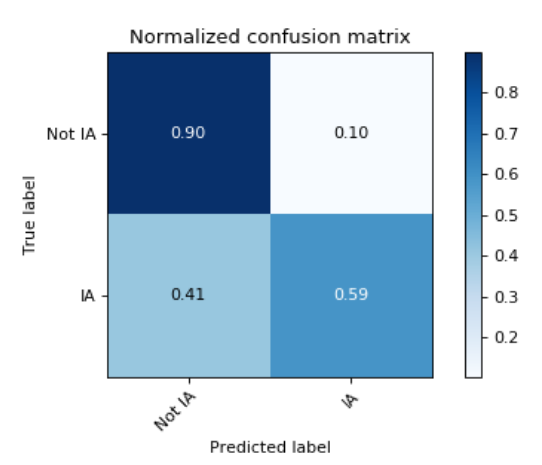
\includegraphics[width=\textwidth]{result_DL1.png}
 			\caption[]%
 			{{\small Valores normalizados.}}    
 		\end{subfigure}
 		\hfill
 		\begin{subfigure}[b]{0.475\textwidth}  
 			\centering 
 			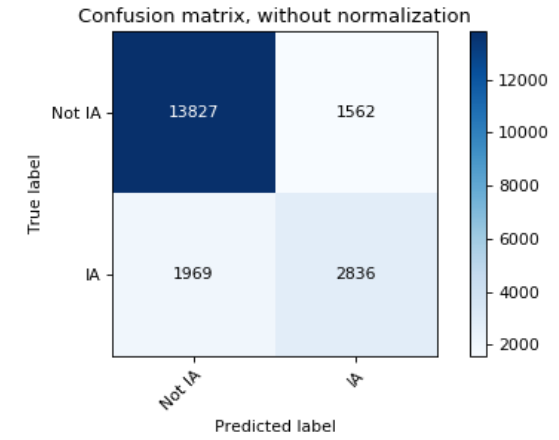
\includegraphics[width=\textwidth]{result_DL2.png}
 			\caption[]%
 			{{\small Valores absolutos.}}    
 		\end{subfigure}
 		\caption[ Matrizes de confusão do modelo final. \textit{Deep Learning}.]
 		{\small Matrizes de confusão do melhor modelo de Deep Learning.} 
 		\label{fig:resultadoDL}
 	\end{figure*}
 
 	Ao compararmos os resultados da figura \ref{fig:resultadoDL} com o da figura \ref{fig:CMEx} percebemos que o modelo de Deep Learning apresentou piora em seu desempenho.
 	
 	Dois motivos podem explicar tais resultados, o primeiro deles é o fato das imagens treinadas não terem sofrido o chamado \textit{data augmentation}, uma técnica que busca aumentar a quantidade de dados treinados e variar suas formas de identificação, focando em rotacionar, deslocar, reduzir e aumentar as figuras. Devido as imagens deste projeto serem gráficos, haveria uma perda de sentido caso os mesmos fossem rotacionados ou deslocados.
 	
 	O segundo motivo é a limitação física que faz com que sejam treinados apenas 1100 objetos astronômicos. Normalmente algoritmos de Deep Learning mostram-se mais vantajosos do que algoritmos de ML devido a grande quantidade de dados que os faz ter um desempenho melhor.
 	
 	Por fim, também foram feitos experimentos envolvendo uma distribuição de dados de $80\%$ para treino de $20\%$ para teste. A análise dessas matrizes de confusão (figuras \ref{fig:DLScuks1} e \ref{fig:DLScuks2}) confirmam que para este problema a aplicação de Deep Learning analisando o formato dos gráficos não se mostra eficiente, reiterando a justificativa da ausência do \textit{data augmentation}.
 	
 	 \begin{figure}[ht]
 		\centering
 		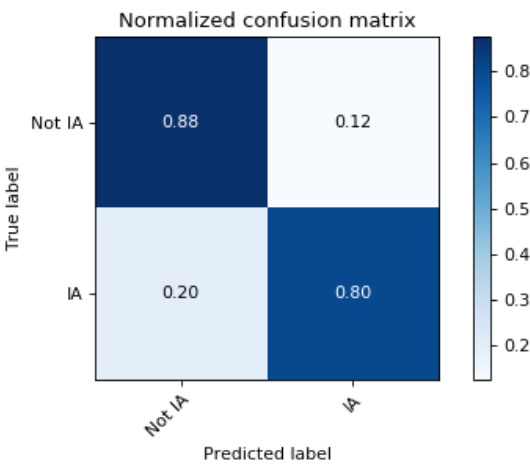
\includegraphics[width=7cm]{dldef.png}
 		\caption{Valores normalizados do modelo DL treinando com 80\% dos dados.}
 		\label{fig:DLScuks1}
 	\end{figure}
 
 	 \begin{figure}[ht]
 		\centering
 		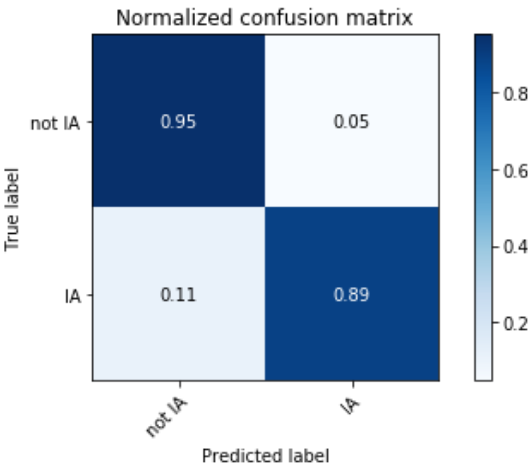
\includegraphics[width=7cm]{cmmarc.png}
 		\caption{Modelo do \textit{pipeline} original treinado com 80\% dos dados.}
 		\label{fig:DLScuks2}
 	\end{figure}

 	
 	
	\newpage
  \chapter{Interpolação através de Processo Gaussiano}
  \label{chap:GP}
  
  	A abordagem feita pelo IF-UFRJ ao usar o Processo Gaussiano foi através da biblioteca \textit{george} \cite{george}. Uma biblioteca focada em avaliar a probabilidade marginal \cite{marginallikelihood} \cite{GPBook} da distribuição dos dados. 
  	
 	Contudo, ao tentar editar alguns parâmetros internos referentes a interpolação nesta biblioteca, como os Kernels ou funções a priori \ref{sec:GP}, houve certa dificuldade ou mesmo impossibilidade de modelá-los da maneira desejada. Como, por exemplo, somar e multiplicar Kernels, sobretudo aqueles não-estacionários (Cap. 3 \cite{GPBook} ).
 	
 	Um motivo que levou o projeto a usar uma outra biblioteca foi a citação do capítulo 4 seção 2 do \citet{GPBook}, argumentando que o Kernel de tipo \textit{Squared Exponential Covariance Funtion} (utilizado no pipeline original) propicia à função interpolada uma suavização irreal para diversos fenômenos físicos, e recomenda usar Kernels do tipo \textit{Matern}. Apesar de a biblioteca \textit{george} também conter esse tipo de Kernel, outras bibliotecas possuíam uma maior possibilidade de modificação de edição. Além do fato de que o tipo \textit{Matern} foi aplicado através da biblioteca \textit{george}, mas não obteve um resultado melhor \ref{tab:materngeorge}.
 	
 	Na seção abaixo serão vistos os tipos de bibliotecas analisadas.
  
	\section{Escolha da Biblioteca}
	
		A biblioteca utilizada no artigo da \citet{lochner} foi a \textit{Gapp}, uma biblioteca para reconstrução de funções usada em outros trabalhos de cosmologia \cite{gapp}.
		
		Entretanto, o próprio pipeline desenvolvido pelo IF-UFRJ já buscava otimizar o artigo original da M. Lochner, logo, este projeto partiu dos estudos já feitos, tendo como ponto de partida a biblioteca \textit{george}.
		
		Vale mencionar também que embora seja possível implementar manualmente os processos gaussianos, as várias bibliotecas disponíveis já possuem especificações e ajustes para os modelos de maneira mais automatizada. As três bibliotecas analisadas foram:
		
		\begin{itemize}
			\item SciKit-Learn
			\item GPflow
			\item PyMC3
		\end{itemize}
		
		Em particular, cada um desses pacotes inclui um conjunto de funções de covariância que podem ser flexivelmente combinadas para descrever adequadamente os padrões específicos dos dados, juntamente aos métodos para ajustar os parâmetros do GP.
		
		A maior parte da análise foi baseada no blog \textit{Domino}, onde vários experimentos foram realizados comparando o desempenho de cada pacote \cite{bibliotecacomp}. 
		
		As minuciosidades destas análises podem ser vistas em todo o projeto realizado no blog citado acima, para não fugir do escopo deste trabalho não serão mencionados mais detalhes sobre a especificidade de cada biblioteca.
		
		Como explicação breve para a escolha final, pode se dizer globalmente que o \textit{scikit-learn} possui uma abordagem mais simples e focada menos nos modelos probabilísticos sofisticados. Enquanto tanto o \textit{GPFlow} quanto o PyMC3 possuem um próprio \textit{backend} computacional dando suporte a esses modelos. Por fim, o motivo da escolha do PyMC3 foi devido a maior comunidade de suporte e ao vasto domínio de estudo da biblioteca. Pois, por ser um pacote de programação probabilística, o PyMC3 abrange mais ferramentas que podem vir a ser úteis no desenvolvimento das distribuições de probabilidade usadas no GP.
		
	\section{Aleatoriedades e \textit{Random Seeds}}
	
	Antes de adentrar nas escolhas dos Kernels, é muito importante explicar o fator da aleatoriedade dentro do projeto. Normalmente a biblioteca PyMC3 realizaria métodos de otimização da função a posteriori em seu GP, entretanto, por ser uma biblioteca que exige um alto custo computacional, foi decidido não executar a linha de código que otimizaria o código em prol de escolher uma função Kernel que melhor faria a interpolação.
	
	Isto não significa que os parâmetros do GP não serão otimizados, eles apenas não irão convergir para um valor final, o que os torna dependentes das condições iniciais estabelecidas internamente pelo computador durante as cadeias de Markov Monte Carlo \cite{MCMC}.
	
	A alternativa para esta escolha de projeto foi comparar determinadas sementes aleatórias \cite{pseudoaleatoriedade}. Através da análise de 11 sementes pôde-se escolher aquelas cujas condições iniciais resultavam em um maior overfitting das interpolações. As figuras das comparações das interpolações de cada semente encontram-se no apêndice \ref{chap:ApendiceB}.
	
	Buscando sempre aquelas sementes que eliminam interpolações constantes e proporcionam um \textit{overfitting}, as melhores foram:
	
	\begin{itemize}
	\item Random Seed 8, possuiu overfitting muito alto.
	\item Random Seed 6, possuiu também um alto overfitting.
	\item Random Seed 5, em troca de uma margem de erro menor, seu overfitting também é reduzido.
	\item Random Seed 4, comportamento buscando reduzir os erros com overfitting e corrigindo o problema dos valores constantes.
	\item Random Seed 9, a melhor combinação entre overfitting e erro não possuindo interpolações constantes.
	\item Random Seed 7, possui uma boa interpolação mas não corrige o problema de interpolações constantes.
	\end{itemize}
	
	Por fim, foram escolhidas duas delas para as interpolações finais, as sementes 4 e 9.
	
	\section{\textit{Kernel Functions}}
	
	Para escolher as funções Kernel que seriam utilizadas nas interpolações, foi seguido o suporte da biblioteca PyMC3 \cite{pymc}. Nesse suporte existem diferentes maneiras de interpolações e análises sobre como os Kernels afetam diretamente no formato das funções.
	
	A partir dos dados da referência acima, foram escolhidos os seguintes Kernels para as interpolações:
	
	\begin{itemize}
		\item Exponencial quadrática:
			\begin{equation}
			k(x, x') = \mathrm{exp}\left[ -\frac{(x - x')^2}{2 \ell^2} \right]
			\end{equation}
		\item Racional quadrática:
			\begin{equation}
			k(x, x') = \left(1 + \frac{(x - x')^2}{2\alpha\ell^2} \right)^{-\alpha}
			\end{equation}
		\item \textit{Matern} 5/2:
			\begin{equation}
			k(x, x') = \left(1 + \frac{\sqrt{5(x - x')^2}}{\ell} +
			\frac{5(x-x')^2}{3\ell^2}\right)
			\mathrm{exp}\left[ - \frac{\sqrt{5(x - x')^2}}{\ell} \right]
			\end{equation}
		\item \textit{Matern} 3/2:
			\begin{equation}
			k(x, x') = \left(1 + \frac{\sqrt{3(x - x')^2}}{\ell}\right)
			\mathrm{exp}\left[ - \frac{\sqrt{3(x - x')^2}}{\ell} \right]
			\end{equation}	
	\end{itemize}
	
	Nestas funções temos $x$ e $x'$ como os valores das abscissas e $\alpha$ e $l$ como hiperparâmetros a serem ajustados. Empiricamente percebeu-se que o $l$ possui um efeito de aumentar overfitting em troca do aumento do erro da interpolação.
	
	Esses hiperparâmetros podem assumir valores como funções de distribuições probabilísticas ou como  constantes. Após diversos testes utilizando constantes, foi notório que os melhores resultados foram obtidos usando distribuições. Outro fator que levou a essa escolha, foram os exemplos oferecidos no suporte da biblioteca PyMC3 \cite{pymcex} \cite{pymcgs}. 
	
	No apêndice \ref{chap:ApendiceB} são ilustradas as interpolações realizadas para escolher qual Kernel seria utilizado. Os critérios principais para a  escolha foram evitar interpolações constantes e buscar overfitting. Como resultado, os dois melhores Kernels foram o \textit{Matern} 3/2 e o \textit{Matern} 5/2; uma conclusão alinhada com a teoria exposta no capítulo 4 seção 2 do \citet{GPBook}.
	
	

			
	\section{Demais Observações}
	
	Antes de adentrar nos resultados das Interpolações, duas observações importantes são feitas.
	
	A primeira é a solução para o problema de possíveis valores negativos. Por mais que tal abordagem não tenha sido adotada neste trabalho, devido à tentativa de deixar o código com menos custo computacional possível; para trabalhos futuros nos quais deseje-se impossibilitar interpolações com valores negativos, o uso de uma \textit{mean function} não-negativa resolve este problema \cite{pymccont}.
	
	Vários tipos de funções que atendem esse pré-requisito estão descritos no \citet{pymccont}.
	
	Um exemplo pode ser a \textit{Half-Cauchy log-likelihood}.
	
	\begin{equation}
		f(x \mid \beta) = \frac{2}{\pi \beta [1 + (\frac{x}{\beta})^2]}
	\end{equation}
	
	\begin{figure}[ht]
		\centering
		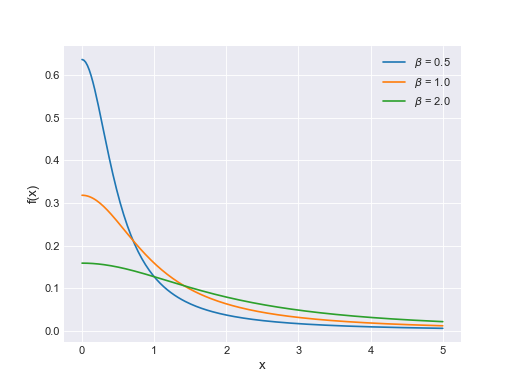
\includegraphics[width=12cm]{halfcauchy.png}
		\caption{Exemplo de distribuição com valores não-negativos.}
		\label{fig:HalfCauchy}
	\end{figure}
			
			
	A segunda observação é o uso da função Matern dentro da própria biblioteca usada no pipeline original do \textit{george}.
	
	Os resultados da troca do Kernel \textit{ExpQuadr} pelo \textit{Matern} 5/2 na biblioteca \textit{george} podem ser vistos em \ref{tab:materngeorge} e \ref{fig:CMmaterngeorge}
	
	\begin{table}[h!]
	
	\begin{center}	
		\small\addtolength{\tabcolsep}{-5pt}
	\begin{tabular}{|l|c|c|c|}
		\hline
		
		Fold & \textbf{AUC} & \textbf{AP} & \textbf{Default scikit}\\
		
		\hline
\small{Fold 1 }&   94,79\%& 83,15\%& 88,88\%\\
\small{Fold 2 }&   94,42\%& 81,28\%& 88,50\%\\
\small{Fold 3 }&   94,32\%& 81,86\%& 88,74\%\\
\small{Fold 4 }&   93,92\%& 80,44\%& 88,26\%\\
\small{Fold 5 }&   94,53\%& 83,51\%& 88,67\%\\
\small{Fold 6 }&   93,92\%& 79,85\%& 88,32\%\\
\small{Fold 7 }&   94,09\%& 82,05\%& 88,72\%\\
\small{Fold 8 }&   94,10\%& 81,51\%& 88,22\%\\
\small{Fold 9 }&   93,74\%& 82,14\%& 88,18\%\\
\small{Fold 10} &  94,04\%& 82,67\%& 88,43\%\\
\small{Fold 11} &  94,82\%& 83,75\%& 89,33\%\\
\small{Fold 12} &  93,97\%& 83,03\%& 89,14\%\\
\small{Fold 13} &  94,36\%& 82,31\%& 88,35\%\\
\small{Fold 14} &  94,38\%& 83,42\%& 88,56\%\\
\small{Fold 15} &  93,83\%& 81,28\%& 88,01\%\\
\small{Fold 16} &  94,12\%& 82,24\%& 88,29\%\\
\small{Fold 17} &  94,72\%& 83,30\%& 88,90\%\\
\small{Fold 18} &  94,21\%& 82,23\%& 88,63\%\\
\small{Fold 19} &  94,26\%& 81,63\%& 88,38\%\\
		\hline
		\hline
		\textbf{Média} &  \textbf{94,24\%} & \textbf{82,19\%} & \textbf{88,55\%} \\
		\hline
		
	\end{tabular}
	\end{center}
	\caption{Resultados do Kernel \textit{Mattern 5/2} pela biblioteca \textit{george}.}
	\label{tab:materngeorge}
	\end{table}
	
	A justificativa para tal desempenho ser pior pode ser atribuída aos hiperparâmetros terem sido constantes e não distribuições. Em contrapartida, poderia ser concluído que o uso do Matern é inferior ao do \textit{Exp Quadr} caso analisasse apenas o resultado do \textit{george}. Todavia, ao realizar comparações dentro de uma biblioteca com mais suporte, é visivelmente notada a melhora ao interpolar usando o Kernel proposto do que o antigo \ref{fig:GPResult}.
	
	
	\section{Resultados das Interpolações}
	
	O resultado global das interpolações não pôde ser concluído devido a um erro de processamento de código, mais precisamente um \textit{memory leak} interno durante a execução dos modelos do PyMC3 em \textit{loop}. A explicação e detalhamento desse erro será apresentado na seção a seguir. 
	
	Nesta seção serão apresentados apenas alguns exemplos de comparação de interpolação entre os algoritmos, justificando o porquê de se esperar que caso o processamento de todos os dados fosse concluido, provavelmente obter-se-iam resultados melhores.
	
			\begin{figure*}
			\centering
			\begin{subfigure}[b]{0.475\textwidth}
				\centering
				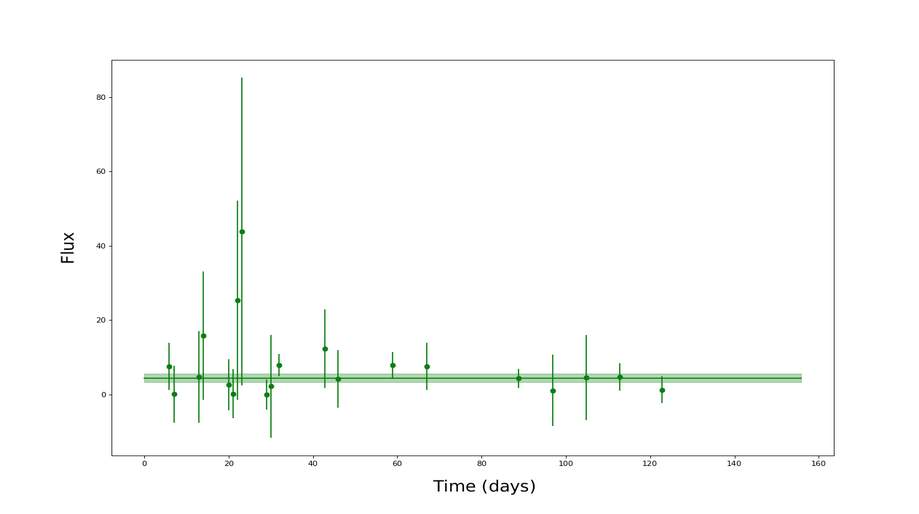
\includegraphics[width=\textwidth]{Ex_reta.png}
				\caption[]%
				{{\small Pipeline original}}    
			\end{subfigure}
			\hfill
			\begin{subfigure}[b]{0.475\textwidth}  
				\centering 
				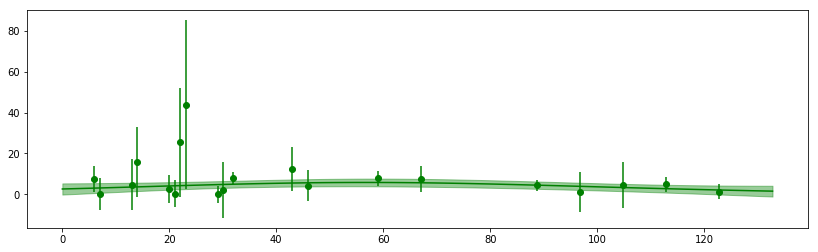
\includegraphics[width=\textwidth]{SN013742_pymc_eq.png}
				\caption[]%
				{{\small PyMC3 Exponential Quadratic semente 9}}    
			\end{subfigure}
			\vskip\baselineskip
			\begin{subfigure}[b]{0.475\textwidth}   
				\centering 
				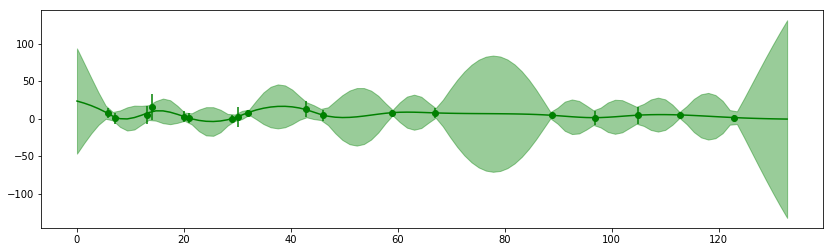
\includegraphics[width=\textwidth]{SN013742_pymc_m52_6.png}
				\caption[]%
				{{\small PyMC3 Matern 5/2 semente 6, overfitting}}    
			\end{subfigure}
			\quad
			\begin{subfigure}[b]{0.475\textwidth}   
				\centering 
				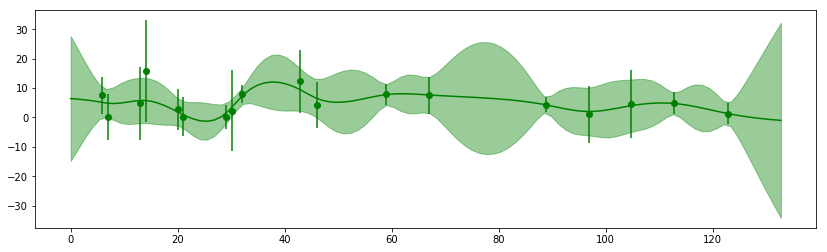
\includegraphics[width=\textwidth]{SN013742_pymc_m52_9.png}
				\caption[]%
				{{\small PyMC3 Matern 5/2 semente 9, overfitting}}    
			\end{subfigure}
			\vskip\baselineskip
			\begin{subfigure}[b]{0.475\textwidth}   
				\centering 
				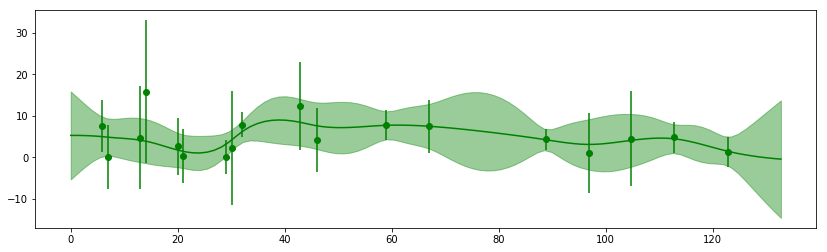
\includegraphics[width=\textwidth]{SN013742_pymc_m52_6_noOF.png}
				\caption[]%
				{{\small PyMC3 Matern 5/2 semente 6, menos overfitting}}    
			\end{subfigure}
			\quad
			\begin{subfigure}[b]{0.475\textwidth}   
				\centering 
				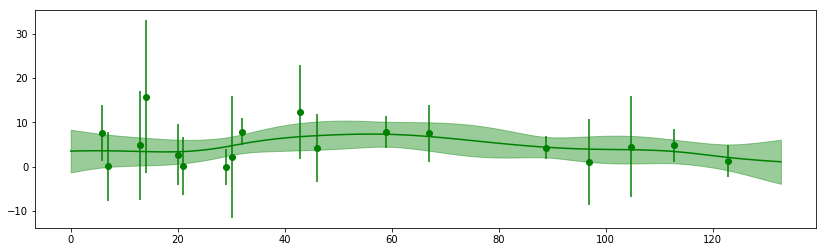
\includegraphics[width=\textwidth]{SN013742_pymc_m52_9_noOF.png}
				\caption[]%
				{{\small PyMC3 Matern 5/2 semente 9, menos overfitting}}    
			\end{subfigure}
			\caption[ Comparação dos resultados finais para um exemplo.]
			{\small Interpolações do objeto SN013742 usando 6 configurações diferentes. Gráfico Fluxo $ \times $ Tempo (dias).} 
			\label{fig:GPResult}
		\end{figure*}
	
	 	\begin{figure*}[h]
		\centering
		\begin{subfigure}[b]{0.475\textwidth}
			\centering
			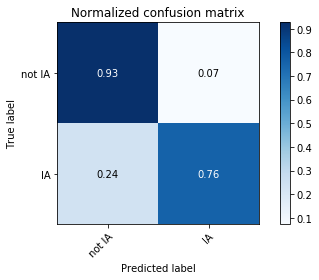
\includegraphics[width=\textwidth]{CM_mat_george_normal.png}
			\caption[]%
			{{\small Valores normalizados.}}    
		\end{subfigure}
		\hfill
		\begin{subfigure}[b]{0.475\textwidth}  
			\centering 
			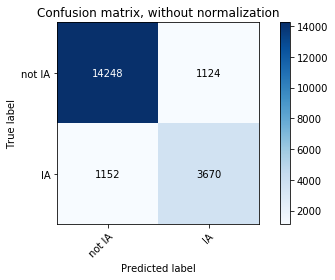
\includegraphics[width=\textwidth]{CM_mat_george_absolut.png}
			\caption[]%
			{{\small Valores absolutos.}}    
		\end{subfigure}
		\caption[ Matrizes de confusão do \textit{Matern 5/2} pela biblioteca \textit{george}.]
		{\small Matrizes de confusão do \textit{Matern 5/2} pela biblioteca \textit{george}.} 
		\label{fig:CMmaterngeorge}
		\end{figure*}

		
		Demais exemplos de comparações estão descritos no \textit{notebook} do apêndice \ref{chap:ApendiceB}.
		
	\section{Identificação e Justificativa do Erro}
	\newpage 

  \chapter{Conclusões}
  \label{chap:Concl}
	\section{Conclusões Finais} 	  
	
	O presente trabalho teve como objetivo buscar otimizações e melhorias nas técnicas de ML dentro dos modelos de classificação de supernovas usando espectroscopia. A partir da análise dos resultados, foi possível verificar que o modelo atual possui uma robustez muito eficaz tendo em vista a pouca quantidade de dados treinados.
	
	Como ponto positivo para o método, este projeto pôde agregar conhecimento testando diferentes abordagens e concluindo que suas aplicações não ofereceriam melhoras ao modelo. Além de averiguar que a robustez do método.
	
	Dentro do escopo de um projeto final, cabe também mencionar a evolução e aquisição de conhecimento do aluno, que ao realizar pesquisas e discutir novas ideias para o algoritmo, teve um aprendizado significativo a medida em que foram sendo descobertas e estudadas novas tecnologias e novos conceitos.
	
	Ao aplicar a estratégia de tratamento de dados removendo os \textit{outliers}, foi possível observar que a diferença dos resultados finais mostrou-se tão pequena que pode ser desprezada, levando a conclusão de que a etapa das transformadas de \textit{wavelets} proporciona ao algoritmo uma robustez significativa, a ponto de que \textit{outliers} 'grosseiros' não comprometeram o modelo.
	
	Em relação ao Deep Learning concluiu-se que no local onde as redes neurais convolucionais foram aplicadas, essa técnica não se mostrou eficaz devido aos modelos serem treinados com apenas um dezenove avos dos dados. Além de concluir que a ausência de um possível \textit{data augmentation} compromete o desempenho mesmo quando são utilizados 80\% dos dados para treino.
	
	\newpage
	
	Por fim, a abordagem principal que foi a busca de uma melhor execução do Processo Gaussiano não pôde ser concluída devido a problemas que fugiram da natureza do projeto. Entretanto, a partir da análise de outros métodos e dos resultados das interpolações dos gráficos através do Kernel \textit{Mattern 5/2} pelo \textit{george}, conclui-se que o método atual já se encontra bem otimizado, sustentado principalmente pela robustez que a transformada de \textit{wavelets} oferece ao modelo.  
	
		
	\section{Trabalhos Futuros} 
		
	Em relação à utilização de aprendizado de máquina na temática em questão, muitos outros métodos são usados para a identificação de objetos astronômicos para demais fins \cite{sooknunan}. Tendo em vista esses outros objetivos, o trabalho aqui desenvolvido mostra-se útil para projetar novas ideias nessas outras abordagens.
	
	Em relação ao erro de \textit{memory leak}, a resolução fica em aberto para trabalhos futuros que busquem finalizar a ideia aqui já construída. Visto que a parte árdua de identificar o problema já foi feita, o mesmo pode ser publicado em repositórios e comunidades de programadores buscando suporte direcionado.
	
	Sobre as outras bibliotecas estudadas para realizar a interpolação, após a análise e detalhamento de cada uma delas e suas propriedades \cite{bibliotecacomp}, elas podem se mostrar interessantes em trabalhos cujo uso de Processo Gaussiano seja necessário.
	
	Após a utilização da biblioteca PyMC3, apesar do problema ocorrido, ela se mostrou extremamente eficaz e matematicamente completa, estando alinhada com os conceitos estatísticos proporcionando uma flexibilidade na modelagem das distribuições. Logo, é aconselhável que novos interessados no projeto usem a biblioteca, devido ao seu grande suporte que facilita o entendimento teórico. Assim como àqueles que já possuem determinado conhecimento e queiram tentar modelos mais específicos e customizados.
		  

  \backmatter
  \bibliographystyle{coppe-unsrt}
  \bibliography{bibliografia}

  \appendix
  \chapter{Repositório do Código}
  \label{chap:Apendice}
  
  Todo o código desenvolvido encontra-se disponível no repositório público do \textit{GitHub}, a fim de poder ser desenvolvido e modificado por qualquer pessoa que deseje contribuir ou estudar este projeto, podendo ser acessado no seguinte link: \href{https://github.com/FelipeMFO/supernova_identification}{https://github.com/FelipeMFO/supernova\_identification}.
  
  \chapter{Avaliação das Interpolações}
  \label{chap:ApendiceB}
  
  Dentro do repositório citado no apêndice \ref{chap:Apendice}, um \textit{notebook} em especial possui as diversas interpolações feitas para avaliar de maneira empírica quais métodos e quais \textit{random seeds} se mostraram mais eficazes. O arquivo é o \href{https://github.com/FelipeMFO/supernova_identification/blob/master/src_and_notebooks/processing/GP_evaluation.ipynb}{https://github.com/FelipeMFO/supernova\_identification/blob/master/src\_and\_notebooks/processing/GP\_evaluation.ipynb}.
  
  
\end{document}
%% 
%%
%% End of file `example.tex'.
